\chapter{An Asymmetric Mode-Matching Model}\label{ch:m12}
As we have discussed the split-cylinder resonator is a very accurate and well-researched dielectric measurement method. In our research on the split-cylinder resonator we implemented Janezic's mode-matching model, since it is a widely accepted and well-documented model developed at the renowned American metrology institute NIST. We also manufactured a split-cylinder prototype at our institute's work shop, which confronted us with the limited manufacturing precision of our equipment. Since the mode-matching model assumed a symmetric resonator with two identical cavities at the top and at the bottom, the accuracy of our split-cylinder was very much in doubt. We recognised that a major drawback of the method was the relatively costly production of the cavity. Lower manufacturing cost would allow us to tailor a cylinder to each specimen. This would also circumvent the issues surrounding the large detuning of split-cylinder resonators with thick samples and higher permittivities. Each cavity could be built to have its first TE\st{0np} measurement mode around a certain frequency. This encouraged us to expand and modify the mode-matching model to asymmetric split-cylinders, since the variations in diameter and length of the upper and lower cavities were identified as a potential root of systematic error. For these modifications we had to expand the mode-matching model and change the calibration procedure, both of which we will now derive in this chapter. 
\section{Fields of the Measurement Model}
\begin{figure}
\centering
\begin{tikzpicture}
   %\draw[step=1cm,gray,very thin] (-3,0) grid (13,7.5);
    \node[anchor=south west,inner sep=0] (image) at (0,0) {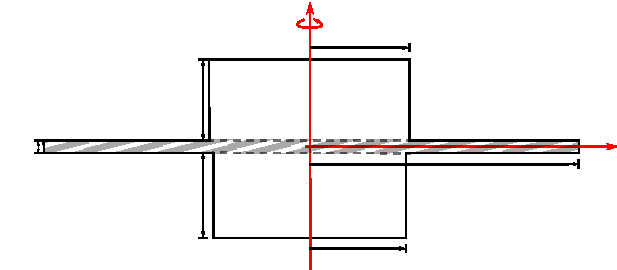
\includegraphics[width=10cm]{split_cylinder_resonator_model.pdf}};
    \draw (5,4.6) node[red] {\textit{z}};
    \draw (10.25,2) node[red] {\textit{$\rho$}};
    \draw (3,2.75) node {$L_u$};
    \draw (3,1.25) node {$L_l$};
    \draw (0.25,2) node {$d$};
    \draw (5.75,3.8) node {$a_u$};
    \draw (5.75,0.1) node {$a_l$};
    \draw (8,1.5) node {$b$};
    
    \draw (3.75,2.75) node[anchor=west] {\scalebox{0.75}{$\mu_0,\epsilon_{lab}$}};
    \draw (3.75,1.25) node[anchor=west]  {\scalebox{0.75}{$\mu_0,\epsilon_{lab}$}};
    \draw (3.75,2) node[anchor=west]  {\scalebox{0.75}{$\mu_0,\epsilon_{s}$}};
\end{tikzpicture}
\caption{Geometry of an asymmetric split-cylinder resonator.}\label{fig:a_SC}
\end{figure}

Janezic \cite{janezic} derived an accurate model for the split-cylinder resonator, which used mode-matching to compute the field configuration in the cavity. Mode-matching is a popular method of computer-aided electro-magnetics \cite{sorrentino, arndt}, which uses the eigenmode expansion of the modes in a region to enforce the boundary conditions at the interface to another region. For the expansion we first need the eigenmodes of each region, so the method requires solutions of the boundary value problem in each region to work. The starting point for our boundary value problem is the electro-magnetic model and geometry of an asymmetric split-cylinder resonator shown in Fig. \ref{fig:a_SC}. The split-cylinder resonator is dielectric measurement method for thin, low-loss dielectric sheets. Its model consists of three open cylindrical cavities that are aligned along a common z-axis. The cavities are an upper-cavity with diameter $2a_u$ and length $L_u$, a sample region with diameter $2b$ and length $d$ and a lower cavity with diameter $2a_l$ and length $L_l$. There two step-discontinuities, one at the interface between upper cavity and sample region and another one between the lower cavity and the sample region. At these interfaces the diameter of the cavity changes abruptly creating a conductive flange at the interface. In terms of materials the cavities are filled with air and the sample region with a linear, homogeneous, isotropic and lossy dielectric, so $\mu=\mu_0$ and $\epsilon_{lab}=1.00055\,\epsilon_0$ may be assumed for the cavities and $\mu=\mu_0$ and $\underline{\epsilon_s}=(\epsilon_r-j\epsilon_r\tan\delta)\epsilon_0$ for the sample region \cite{phillips}. The entire cavity is enclosed by a good conductor with conductance $\sigma$.

To compute the mode-matching model our first step is to solve the boundary value problem of the cylindrical cavities. The wave equation of time-harmonic electric fields in a source- free medium is
\begin{equation}
\nabla^2\vec{E}=\gamma^2\vec{E} \quad\text{with}\quad \gamma=j\omega\mu_0(\sigma+j\omega\epsilon)=j\omega\mu_0(\omega\epsilon''+j\omega\epsilon ')=\omega^2\mu_0\epsilon '(j\tan\delta - 1)\text{,}
\end{equation}
where $\gamma$ is the separation constant of the partial differential equation. We assume that the influence the dielectrics loss of the low-loss dielectrics on the field configurations is negligible, i.e. $\tan\delta=0$,
\begin{equation}\label{eq:wave}
\nabla^2\vec{E}=-k^2\vec{E} \quad \text{and} \quad k=\omega^2\mu_0\epsilon '\text{.}
\end{equation}
From Equation \eqref{eq:wave} the TE and TM eigenmodes of a cylindrical coordinate system can be obtained, of which we are only interested in the TE modes. Using an electric vector potential $\vec{E}=\nabla\times\vec{F}$ and $\vec{F}=F_z\vec{e_z}$ solutions for the TE modes of the wave equation in cylindrical coordinates can be found
\begin{gather}
F_z=\left(A_1J_m(h_n\rho)+B_1Y_m(h_n\rho)\right)\left(C_2\cos(m\phi)+D_2\sin(m\phi)\right)\left(A_3\cos(p_nz)+B_3sin(p_nz)\right)\text{,}\\
k^2=h_n^2+p_n^2\text{,}
\end{gather}
where $J_m$ and $Y_m$ are the mth order Bessel function of the first and second kind, and $A_1$, $B_1$, $C_2$, $D_2$, $A_3$ and $B_3$ are constants. With the curl of $\vec{F}$ we also yield the $\phi$ component of the electric field $E_\phi$
\begin{equation}\begin{split}
E_\phi(\rho,\phi,z)=\frac{1}{\epsilon}\frac{\partial F_z}{\partial\rho}=\frac{1}{\epsilon}\left(A_1h_nJ'_m(h_n\rho)+B_1h_nY'_m(h_n\rho)\right)\left(C_2\cos(m\phi)+D_2\sin(m\phi)\right) \\ \times\left(A_3\cos(p_nz)+B_3sin(p_nz)\right)\text{,}\end{split}
\end{equation}
where $'$ indicate the derivatives of the functions \cite{balanis}. We determine the constants using simplified boundary conditions. We assume that the cavity walls are perfect electric conductors with $\vec{n}\times\vec{E}=\vec{0}$ on the cavity walls. We neglect the influence of lossy walls on the field configuration and we will re-introduce the cavity losses in the loss calculations. A widely accepted simplification that introduces only a minor error in the resonant frequency \cite{collin}. Furthermore, we are only interested in the TE\st{0n} modes of the cavity and since all our cavities are aligned along a common z-axis the TE\st{0n} modes at each interface are orthogonal to all other modes but the TE\st{0n} modes in the other cavity. This special property allows us to expand the fields in the entire cavity in terms of TE\st{0n} modes only, i.e. $\vec{E}=\sum_{n=1}^{\infty}E_{\phi,TE0n}\vec{e_\phi}$. 
The fields in the entire cavity therefore must satisfy:
\begin{enumerate}
\item Azimuthal symmetry of all modes $\Rightarrow m=0 \ \text{and}\ J'_{m=0}(h_n\rho)=-J_1(h_n\rho)$, due to one of the recurrence relations of the Bessel functions
\item Finite fields in the entire cavity $\lim_{\rho\rightarrow 0}Y_m'(h_n\rho)=\lim_{\rho\rightarrow 0}\{Y_{m-1}(h_n\rho)-Y_{m+1}(h_n\rho)\}\rightarrow \infty \Rightarrow B_1=0$
\end{enumerate}
\begin{equation}\label{eq:sol_simple}
E_{\phi}(\rho,z)=\sum\limits_{n=1}^{\infty} \frac{A_nh_n}{\epsilon}J_1(h_n\rho)[A_3\cos(p_nz)+B_3\sin(p_nz)]
\end{equation}
With the simplified solution of Equation \eqref{eq:sol_simple} we can solve the boundary value problem in each cavity with respect to the cavity walls.

Solving the \textbf{upper-cavity} boundary value problem
\begin{gather}
\vec{E}\left(\rho=a_u,\frac{d}{2}\leq z\leq\frac{d}{2}+L_u\right)=\vec{0}\\
\vec{E}\left(0\leq\rho\leq a_u,z=\frac{d}{2}+L_u\right)=\vec{0}\\
\end{gather}
we find a solution for the electric field in the upper cavity
\begin{align}\label{eq:e_u}
E_{\phi,u}(\rho,z)&=\sum\limits_{n=1}^{\infty} A_nU_nJ_1(h_{n,u}\rho)\sin(p_{n,u}\left(L_u+\frac{d}{2}-z\right)), &\scriptstyle (0\leq\rho\leq a_u)\wedge\left(\frac{d}{2}\leq z\leq\frac{d}{2}+L_u\right)
\end{align}
where
\begin{equation}
h_{n,u}=\{\forall h_n\in\mathbb{R}^+:J_1(h_na_u)=0\}\text{.}
\end{equation}
Using this solution we calculate the magnetic fields in the upper cavity,
\begin{align}\label{eq:h_u}
H_{\rho,u}(\rho,z)&=\frac{1}{j\omega\mu_0}\frac{\partial E_{\phi,u}}{\partial z}\\&=\sum\limits_{n=1}^{\infty}\frac{-p_{n,u}}{j\omega\mu_0}A_nU_nJ_1(h_{n,u}\rho)\cos(p_{n,u}\left(L_u+\frac{d}{2}-z\right)),&\scriptstyle\left(0\leq\rho\leq a_u\right)\wedge\left(\frac{d}{2}\leq z\leq\frac{d}{2}+L_u\right)\\
H_{z,u}(\rho,z)&=\frac{-1}{j\omega\mu_0}\left(\frac{1}{\rho}E_{\phi,u}+\frac{\partial E_{\phi,u}}{\partial\rho}\right)\\&=\frac{-1}{j\omega\mu_0}\sum\limits_{n=1}^\infty A_nU_nh_{n,u}J_0(h_{n,u}\rho)\sin(p_{n,u}\left(L_u+\frac{d}{2}-z\right)),&\scriptstyle(0\leq\rho\leq a_u)\wedge\left(\frac{d}{2}\leq z\leq\frac{d}{2}+L_u\right)
\end{align}
In a similar fashion the boundary value of the \textbf{sample region}
\begin{gather}
\vec{E}\left(\rho=b,-\frac{d}{2}\leq z\leq\frac{d}{2}\right)=\vec{0}
\end{gather}
yields the electric field in the sample region
\begin{align}\label{eq:e_s}
E_{\phi,s}(\rho,z)&=\sum\limits_{m=1}^{\infty} J_1(h_{m,s}\rho)\left(B_mV_m\cos(p_{m,s}z)+C_mW_m\sin(p_{m,s}z)\right),&\scriptstyle(0\leq\rho\leq b)\wedge\left(-\frac{d}{2}\leq z\leq\frac{d}{2}\right)
\end{align}
where
\begin{equation}
h_{m,s}=\{\forall h_m\in\mathbb{R}^+:J_1(h_mb)=0\}\text{.}
\end{equation}
Again, the solution allows us to calculate the magnetic field, so in the sample region we obtain
\begin{align}\label{eq:h_s}
H_{\rho,s}(\rho,z)&=\frac{1}{j\omega\mu_0}\frac{\partial E_{\phi,s}}{\partial z}\\&=\sum\limits_{m=1}^{\infty}\frac{p_{m,s}}{j\omega\mu_0}J_1(h_{m,s}\rho)\left(-B_mV_m\sin(p_{m,s}z)+C_mW_m\cos(p_{m,s}z)\right),&\scriptstyle(0\leq\rho\leq b)\wedge\left(-\frac{d}{2}\leq z\leq\frac{d}{2}\right)\\
H_{z,s}(\rho,z)&=-\frac{1}{j\omega\mu_0}\left(\frac{1}{\rho}E_{\phi,s}+\frac{\partial E_{\phi,s}}{\partial\rho}\right)\\&=\sum\limits_{m=1}^\infty \frac{-h_{m,s}}{j\omega\mu_0}J_0(h_{m,s}\rho)\left(B_mV_m\cos(p_{m,s}z)+C_mW_m\sin(p_{m,s}z))\right), &\scriptstyle((0\leq\rho\leq b)\wedge\left(-\frac{d}{2}\leq z\leq\frac{d}{2}\right)
\end{align}
Lastly, the boundary values of the \textbf{lower cavity}
\begin{gather}
\vec{E}\left(\rho=a_l,-\frac{d}{2}\leq z\leq-\frac{d}{2}-L_l\right)=\vec{0}\\
\vec{E}\left(0\leq\rho\leq a_l,z=-\frac{d}{2}-L_u\right)=\vec{0}
\end{gather}
yield a very similar result for the electric field in the lower cavity as in the case of the upper cavity
\begin{align}\label{eq:e_l}
E_{\phi,l}(\rho,z)&=\sum\limits_{p=1}^{\infty} D_pL_pJ_1(h_{p,l}\rho)\sin(p_{p,l}\left(z+L_l+\frac{d}{2}\right)), & \scriptstyle(0\leq\rho\leq a_l)\wedge\left(-\frac{d}{2}-L_l\leq z\leq-\frac{d}{2}\right)
\end{align}
where
\begin{equation}
h_{p,l}=\{\forall h_p\in\mathbb{R}^+:J_1(h_pa_l)=0\}\text{.}
\end{equation}
Similarly, we yield the following for the magnetic field in the lower cavity
\begin{align}\label{eq:h_l}
H_{\rho,l}(\rho,z)&=\frac{1}{j\omega\mu_0}\frac{\partial E_{\phi,l}}{\partial z}\\&=\sum\limits_{p=1}^{\infty}\frac{p_{p,l}}{j\omega\mu_0}D_pL_pJ_1(h_{p,l}\rho)\cos(p_{p,l}\left(z+\frac{d}{2}+L_l\right)), &\scriptstyle(0\leq\rho\leq a_l)\wedge\left(-\frac{d}{2}-L_l\leq z\leq-\frac{d}{2}\right)\\
H_{z,l}(\rho,z)&=\frac{-1}{j\omega\mu_0}\left(\frac{1}{\rho}E_{\phi,l}+\frac{\partial E_{\phi,l}}{\partial\rho}\right)\\&=\frac{-1}{j\omega\mu_0}\sum\limits_{p=1}^\infty D_pL_ph_{p,l}J_0(h_{p,l}\rho)\sin(p_{p,l}\left(z+\frac{d}{2}+L_l\right)), &\scriptstyle(0\leq\rho\leq a_l)\wedge\left(-\frac{d}{2}-L_l\leq z\leq-\frac{d}{2}\right)
\end{align}
For the derivations of the electric fields we merged all constants to common coefficients $A_n$, $B_m$, $C_m$ and $D_p$, and combined them with conditioning coefficient $U_n$, $V_m$, $W_m$ and $D_p$, which will be useful later on.
\subsection{Mode-Matching at the Cavity Interfaces}
With the eigenmode expansion of TE\st{0n} modes in each region at hand, we can now compute the field in the entire cavity. To achieve this we must choose the eigenmode expansion coefficients $A_n$, $B_m$, $C_m$ and $D_p$ as such that the boundary conditions at the interfaces are enforced. The key to this expansion is the orthogonality of the transverse electric fields in a lossless waveguide \cite[Ch. 5.1]{collinFT}. The orthogonality relation of the transverse electro-magnetic fields is the scalar product of the transverse electric field of mode $n$ and the transverse magnetic field of mode $m$, in case of the upper cavity this is the following relation:
\begin{equation}\label{eq:o_u}
\int\limits_0^{2\pi}\int\limits_0^{a_u} E_{\phi,u}^{(n)}H_{\rho,u}^{(m)} \rho d\rho d\phi=K_1\delta_{mm}
\end{equation}
For the sample region the orthogonality relation is
\begin{equation}\label{eq:o_s}
\int\limits_0^{2\pi}\int\limits_0^{b} E_{\phi,s}^{(n)}H_{\rho,s}^{(m)} \rho d\rho d\phi=K_2\delta_{mm}
\end{equation}
and for the lower cavity it is
\begin{equation}\label{eq:o_l}
\int\limits_0^{2\pi}\int\limits_0^{a_l} E_{\phi,l}^{(n)}H_{\rho,l}^{(m)} \rho d\rho d\phi=K_3\delta_{mm}\text{,}
\end{equation}
where $K_1$, $K_2$ and $K_3$ are constants.

The first boundary conditions we need to enforce are at the interface between the upper cavity and the sample region. We demand that the tangential electric field must be continuous across the opening and zero along the perfectly conductive flange, so
\begin{align}\label{eq:bc_1}
E_{\phi,s}\left(\rho,z=\frac{d}{2}\right)= \begin{cases}
    E_{\phi,u}(\rho,z=\frac{d}{2}) , & 0\leq\rho\leq a_u\\
    0, & a_u\leq\rho\leq b
  \end{cases}
\end{align}
must apply. If we insert Equation \eqref{eq:e_l} and \eqref{eq:e_s} into \eqref{eq:bc_1}, we yield
\begin{gather}\label{eq:bc_12}
\sum_{m'=1}^\infty J_1(h_{m',s}\rho)\left\{B_{m'}V_{m'}\cos\left(p_{m',s}\frac{d}{2}\right)+C_{m'}W_{m'}\sin\left(p_{m',s}\frac{d}{2}\right)\right\}=\nonumber\\ \begin{cases}
	\sum_{n=1}^\infty A_nU_nJ_1(h_{n,u}sin(p_{n,u}L_u),&0\leq\rho\leq a_u\\0,& a_u\leq\rho\leq b
\end{cases}
\end{gather}
Next we calculate the scalar product of each side of Equation \eqref{eq:bc_12} and the tangential magnetic field of a mode m from the sample region, for which we multiply both sides with $H_{\rho,s}^{(m)}$  and integrate the expression over the entire surface of the boundary. Due to the orthogonality of the electro-magnetic modes we yield
\begin{gather}
\sum_{n=1}^\infty A_nU_n\frac{a_uh_{n,u}}{h_{m,s}^2-h_{n,u}^2}J_0(h_{n,u}a_u)J_1(h_{m,s}a_u)\sin(p_{n,u}L_u)\nonumber\\=\frac{b^2}{2}J_0(h_{m,s}b)^2\left\{ B_mV_m\cos(p_{m,s}\frac{d}{2})+C_mW_m\sin(p_{m,s}\frac{d}{2})\right\}\text{.}\label{eq:mm_1}
\end{gather}
We also expect the tangential magnetic field to be continuous across the interface of the upper cavity with the sample region, this implies
\begin{equation}\label{eq:bc_2}
H_{\rho,s}\left(\rho,z=\frac{d}{2}\right)= H_{\rho,u}\left(\rho,z=\frac{d}{2}\right),\qquad 0\leq\rho\leq a_u
\end{equation}
As before we insert the eigenmode expansions \eqref{eq:h_u}\eqref{eq:h_s} into the boundary condition \eqref{eq:bc_2} and calculate the scalar product of each side with the tangential electric field of a mode $n$ from the upper cavity. We achieve this by multiplying both sides with $E_{\phi,u}^{(n)}$ and integrating the expression over the surface of the opening.
\begin{gather}
A_nU_np_{n,u}\frac{a_u^2}{2}J_0^2(h_{n,u}a_u)\cos(p_{n,u}L_u)\nonumber\\=\sum\limits_{m=1}^\infty\frac{a_up_{m,s}h_{n,u}}{h_{m,s}^2-h_{n,u}^2}J_1(h_{m,s}a_u)J_0(h_{n,u}a_u)\left\{B_mV_m\sin(p_{m,s}\frac{d}{2})-C_mW_m\cos(p_{m,s}\frac{d}{2})\right\}\label{eq:mm_2}
\end{gather}
We used the tangential magnetic field from the upper cavity to use both orthogonality relations \eqref{eq:o_u} \eqref{eq:o_s} for the boundary conditions, which is supposed to improve the relative convergence of the mode-matching \cite{janezic}. 

For the interface between sample region and lower cavity we use the same procedure for the boundary conditions. The first boundary condition of the interface between sample region and lower cavity is again the continuity of the tangential electric field across the boundary. The $\phi$ component of the electric field in the sample region is supposed to be continuous across the entire opening at the interface and for $\rho$ larger than $a_l$ it is supposed to become zero due to the perfectly conductive flange. 
\begin{align}\label{eq:bc_3}
E_{\phi,s}\left(\rho,z=-\frac{d}{2}\right)= \begin{cases}
    E_{\phi,l}(\rho,z=-\frac{d}{2}) , & 0\leq\rho\leq a_l\\
    0, & a_l\leq\rho\leq b
  \end{cases}
\end{align}
As for the previous boundary conditions we insert the eigenmode expansions of the electric fields of \eqref{eq:e_s} and \eqref{eq:e_l} into the boundary condition \eqref{eq:bc_3} and calculate the scalar product of both sides and the tangential magnetic field of mode $m$ from the lower cavity. This means we multiply both sides of the expansion with $H_{\rho,s}^{(m)}$ and integrate over the entire surface. In the integration the orthogonality relation of the lower cavity \eqref{eq:o_l} makes all members but one of the series on the right hand side become zero.
\begin{gather}
\sum_{p=1}^\infty D_pL_p\frac{a_lh_{p,l}}{h_{m,s}^2-h_{p,l}^2}J_0(h_{p,l}a_l)J_1(h_{m,s}a_l)\sin(p_{p,l}L_l)\nonumber\\=\frac{b^2}{2}J_0(h_{m,s}b)^2\left\{ B_mV_m\cos(p_{m,s}\frac{d}{2})-C_mW_m\sin(p_{m,s}\frac{d}{2})\right\}\text{.}\label{eq:mm_3}
\end{gather}
The second boundary condition of the interface between sample region and lower cavity is also the last boundary condition of the entire boundary value problem of the resonator. The second boundary condition of the interface is the continuity of the tangential magnetic field between sample region and lower cavity. The $\rho$ component of the magnetic field in the sample region is supposed to be continuous across the boundary to the lower cavity. Unlike the tangential electric field at both interfaces the tangential magnetic field is undefined on the surface of the flange.
\begin{equation}\label{eq:bc_4}
H_{\rho,s}\left(\rho,z=-\frac{d}{2}\right)= H_{\rho,l}\left(\rho,z=-\frac{d}{2}\right),\qquad 0\leq\rho\leq a_l
\end{equation}
Like for previous derivations we insert the eigenmode expansions of the magnetic fields \eqref{eq:h_s} and \eqref{eq:h_l} into the boundary condition of the magnetic field \eqref{eq:bc_4}. To use all orthogonality relations we calculate the scalar product of each side of the expression and the tangential electric field of a mode $p$ from the sample region. The scalar product is calculated by multiplying both side with $E_{\phi,l}^{(p)}$ and integrating each term over the surface of the boundary.
\begin{gather}
D_pL_pp_{p,l}\frac{a_l^2}{2}J_0^2(h_{p,l}a_l)\cos(p_{p,l}L_l)\nonumber\\=\sum\limits_{m=1}^\infty\frac{a_lp_{m,s}h_{p,l}}{h_{m,s}^2-h_{p,l}^2}J_1(h_{m,s}a_l)J_0(h_{p,l}a_l)\left\{B_mV_m\sin(p_{m,s}\frac{d}{2})+C_mW_m\cos(p_{m,s}\frac{d}{2})\right\}\label{eq:mm_4}
\end{gather}

Equations \eqref{eq:mm_1}, \eqref{eq:mm_2}, \eqref{eq:mm_3} and \eqref{eq:mm_4} can be used to compute the eigenmode expansion coefficients $A_n$, $B_m$, $C_m$ and $D_p$. The equations are a system of linear equations for the boundary conditions. The boundary conditions must be fulfilled by every mode, so Eq. \eqref{eq:mm_1} is satisfied by all modes of the sample region, Eq. \eqref{eq:mm_2} is satisfied by all modes of the upper cavity, Eq. \eqref{eq:mm_3} is also satisfied by all modes of the sample region and Eq. \eqref{eq:mm_4} is satisfied by all modes of the lower cavity. Obviously, we have one equation for each eigenmode expansion coefficient, which implies that the system of linear equations is uniquely determined. Any solution of the system of linear equations is a mode of the cavity.

The boundary value problem is solved accurately for an infinite number of modes, which is impractical for any real computation. Luckily, we can approximate the boundary conditions by truncating the eigenmode expansion after a given number of modes. Depending on the problem, the approximation can be relatively accurate and the eigenmode expansion can converge to a good estimate for the field configuration of the cavity. This is the principle of mode-matching! We can freely choose the number of modes for each region for the truncated eigenmode expansion. If we include $N_u$ modes from the upper cavity, $N_s$ odd modes from the sample region, $N_s$ even modes from the sample region and $N_l$ modes from the lower cavity, the result is a system of linear equations with $N_u+2N_s+N_l$ unknowns and $N_u+2N_s+N_l$ equations. The system of linear equations is uniquely determined, so either it has a solution or it has none. It can also be written in matrix form
\begin{equation}\label{eq:matZ}
\mat{Z}\vec{x}=\mat{Z}\begin{bmatrix}\vec{A}\\\vec{B}\\\vec{C}\\\vec{D}\\\end{bmatrix}=\vec{0}
\end{equation}
where $\mat{Z}$ is a $\left((N_u+2N_s+N_l)\times(N_u+2N_s+N_l)\right)$ matrix and $\vec{x}$ are the expansion coefficients of the eigenmode expansion. The members of the matrix are defined in Eq. \eqref{eq:m12}
\begin{equation}\label{eq:m12}
 \mat{Z}=\begin{bmatrix}
  \mat{M_1} & -\mat{M_2} & -\mat{M_3} & \mat{0}\\
  \mat{0} &   -\mat{M_4} & -\mat{M_5} & \mat{M_6}\\
  \mat{M_7} & -\mat{M_8} & -\mat{M_9} & \mat{0}\\
  \mat{0} &   -\mat{M_{10}} & -\mat{M_{11}} & \mat{M_{12}}
 \end{bmatrix}_{(N_u+2N_s+N_l)\times(N_u+2N_s+N_l)}\text{,}
\end{equation}
where $\mat{M_1}\,...\,\mat{M_{12}}$ are the sub-matrices
\begingroup
\allowdisplaybreaks
\begin{align}\label{eq:m12_coeff}
\setlength{\jot}{10pt}
&(\mat{M_1})_{mn}=&U_n\frac{a_uh_{n,u}}{h_{m,s}^2-h_{n,u}^2}J_0(h_{n,u}a_u)J_1(h_{m,s}a_u)\sin(p_{n,u}L_u) \\
&(\mat{M_2})_{mm}=&V_m\frac{b^2}{2}J_0(h_{m,s}b)^2\cos(p_{m,s}\frac{d}{2}) \\
&(\mat{M_3})_{mm}=&W_m\frac{b^2}{2}J_0(h_{m,s}b)^2\sin(p_{m,s}\frac{d}{2}) \\
&(\mat{M_4})_{mm}=&(\mat{M_2})_{mm} \\
&(\mat{M_5})_{mm}=&-(\mat{M_3})_{mm} \\
&(\mat{M_6})_{mp}=&L_p\frac{a_lh_{p,l}}{h_{m,s}^2-h_{p,l}^2}J_0(h_{p,l}a_l)J_1(h_{m,s}a_l)\sin(p_{p,l}L_l) \\
&(\mat{M_7})_{nn}=&U_np_{n,u}\frac{a_u^2}{2}J_0^2(h_{n,u}a_u)\cos(p_{n,u}L_u)\\
&(\mat{M_8})_{nm}=&V_m\frac{a_up_{m,s}h_{n,u}}{h_{m,s}^2-h_{n,u}^2}J_1(h_{m,s}a_u)J_0(h_{n,u}a_u)\sin(p_{m,s}\frac{d}{2})\\
&(\mat{M_9})_{nm}=&-W_m\frac{a_up_{m,s}h_{n,u}}{h_{m,s}^2-h_{n,u}^2}J_1(h_{m,s}a_u)J_0(h_{n,u}a_u)\cos(p_{m,s}\frac{d}{2})\\
&(\mat{M_{10}})_{pm}=&V_m\frac{a_lp_{m,s}h_{p,l}}{h_{m,s}^2-h_{p,l}^2}J_1(h_{m,s}a_l)J_0(h_{p,l}a_l)\sin(p_{m,s}\frac{d}{2})\\
&(\mat{M_{11}})_{pm}=&W_m\frac{a_lp_{m,s}h_{p,l}}{h_{m,s}^2-h_{p,l}^2}J_1(h_{m,s}a_l)J_0(h_{p,l}a_l)\cos(p_{m,s}\frac{d}{2})\\
&(\mat{M_{12}})_{pp}=&L_pp_{p,l}\frac{a_l^2}{2}J_0^2(h_{p,l}a_l)\cos(p_{p,l}L_l)\text{.}
\end{align}
\endgroup
\subsection{Finding Solutions for the M12 Matrix and Computing the \texorpdfstring{$\epsilon_r$}{er}}
Since each solution of the boundary-value problem of the split-cylinder resonator is a mode of the resonator, Equation \eqref{eq:matZ} implies that 
each mode is a solution of the Equation $\mat{Z}\vec{x}=\vec{0}$. Mathematically speaking, this means that each mode lies in the null space of $\mat{Z}$ and conversely that there is no solution, if the nullity of the null space of $\mat{Z}$ is zero. Solutions exist only for certain combinations of the variables of $\mat{Z}$, which are combinations of the following variables
\begin{itemize}
\item the geometry of the resonator $a_u$, $b$, $a_l$, $L_u$ and $L_l$,
\item the number of modes $N_u$, $N_s$ and $N_l$,
\item zeros of Bessel functions $h_{n,u}$, $h_{m,s}$ and $h_{n,l}$,
\item conditioning coefficients $U_n$, $V_m$, $W_m$ and $L_p$,
\item permittivity of the lab environment $\epsilon_{lab}$,
\item and the \textbf{measurement variables} $\epsilon_r$, $f_r$ and $d$.
\end{itemize}
Of all these variables only the measurement variables are relevant for a measurement, since the other variables are constants or are related to the numerical convergence. Another indicator for the existence of a solution is the determinant of $\mat{Z}$, since a homogeneous system of linear equations \eqref{eq:matZ} has a non-zero solution only if $\det(\mat{Z})=0$. Since only the measurement variables vary in our measurements, we can write 
\begin{equation}\label{eq:zeros}
\det(\mat{Z}(f,\epsilon_r,d))=0
\end{equation}
for each solution. For a given sample we can determine the solutions of \eqref{eq:zeros} by finding the zero crossings of a plot of $\det(\mat{Z})$. The permittivity of a specimen $\epsilon_r$ can be determined for given $f$ and $d$, the resonant frequency $f$ can be determined for given $\epsilon_r$ and $d$ and thickness $d$ can be determined for given $f$ and $\epsilon_r$.

To find the roots of the determinant of $\mat{Z}$ we employed root-finding techniques. While Janezic \cite{janezic} suggested using a numerical Newton's method to find the roots of the function, Press \cite{press} stated in his well-known work on numerical methods that Brent's method should be chosen in favour of a numerical Newton's method. Although Newton's method converges quadratically, its global convergence is relatively poor and it needs a continuous function to work. Brent's method on the other hand has a weaker linear convergence, but its robustness and good global convergence make it a good choice as a general purpose root-finding algorithm. Although Newton's method converges quadratically the derivatives of the function needs to be known for this rate of convergence. For numerical derivatives the method converges only with the $\sqrt{2}$, since two evaluations of the function are necessary to compute the derivative. Brent's method has at least linear convergence, so the rate of convergence of Brent's method is only a little lower than that of the numerical Newton's method. It should be noted that Brent's method was also readily available for us, since it is the algorithm behind the root-finding function of \textit{MATLAB, FZERO}.

While finding the right root-finding algorithm was relatively straight forward, finding the actual roots was not. It turned out that the numerical properties of this matrix and maybe the properties of most mode-matching matrices was relatively poor and calculations of the null space and the determinant in general did not give correct results. The matrix Z was found to be very numerically unstable or ill-conditioned. This means that its linear equation system is very sensitive to errors, so a small change in the vector $\vec{x}$ of our equation causes a very large error in our computations. The condition of matrices is quantified using a condition number $\kappa_\infty(\mat{Z})$ and ill-conditioned matrices have very high condition numbers. For these very high condition numbers the sensitivity of the matrices to errors becomes so high that the limited precision of the floating point operations on our computer make the result inaccurate. According to Golub \cite{golub}, the unit round-off error $u$ multiplied with the condition number $\kappa_\infty(\mat{A})$ is an estimate for the numerical error of a solution of a linear system of equations
\begin{equation}\label{eq:cond}
\frac{\lVert\vec{\hat{x}}-\vec{x}\rVert_\infty}{\lVert \vec{x}\rVert_\infty}\approx u\kappa_\infty(\mat{A})\text{,}
\end{equation}
where $\lVert\cdot\rVert_\infty$ is the infinity norm of the vector. We found that the condition number of the matrix $\mat{Z}$ exceeded \num{e100} around a solution of the matrix. For the unit round-off error of double precision floating numbers of approximately \num{e-16}, Eq. \eqref{eq:cond} would have predicted an accuracy of $u\kappa_\infty(\mat{A})=\num{e84}$! Apparently, the matrix is too ill-conditioned for any meaningful calculation.

To improve the accuracy of the calculations special transformations called pre-conditioners must be used to lower the condition number of the matrix. In his PhD thesis Janezic decided to use a simple scaling matrix to reduce the condition number. By multiplying each column with a scaling coefficient, he was able to reduce the conditioning number substantially. We observed that the condition number of a matrix around a solution was reduced from \num{e100} down to \num{e20}. Golub's estimate made us expect a relatively large error of \num{e4}, but the results with his pre-conditioner were generally very good and we could not observe any lack of accuracy. Since the condition number was still very large, we tried to change from this pre-conditioner to another pre-conditioning algorithm to improve the performance. Our trials were unsuccessful and the mathematical background of these issues were unknown to us, so we decided to use Janezic's pre-conditioner with the same conditioning coefficients for the even and the odd modes of the sample region:
\begin{align}
U_n &= \frac{p_{N_u,u}}{\cosh(\Im(p_{n,u})L_u)}\\
V_m &= \frac{p_{N_s,s}}{\cosh(\Im(p_{m,s})\frac{d}{2})}\\
W_m &= \frac{p_{N_s,s}}{\cosh(\Im(p_{m,s})\frac{d}{2})}\\
L_p &= \frac{p_{N_l,l}}{\cosh(\Im(p_{p,l})L_l)}
\end{align}
\subsection{Choosing the Right Measurement Modes}
With the conditioning problem out of the way, we can determine the modes of the cavity using a root-finding technique. As we have already explained, each root of the determinant $\det(\mat{Z}(f,\epsilon_r,d))$ has a solution of the equation system $\mat{Z}\vec{x}=\vec{0}$. The solutions, which are the eigenmode expansion coefficients $A_n$, $B_m$, $C_m$ and $D_p$, are the basis of the null space of $\mat{Z}$, which has as many dimensions as there are solutions for the matrix. In most cases each matrix has only one solution, but if there are degenerate modes the matrix may have multiple solutions. Each solution was supposed to be a mode of the split-cylinder, but experience showed that not every root of $\det(\mat{Z})$ was in fact a real mode of the cavity. In our computations many faulty modes occurred as well that were a solution of the numerical matrix $\mat{Z}$ but not of the real boundary value problem. We suspected that the finite numerical accuracy caused problems with the computation of the determinant, so we developed conditions for the modes in our software to filter faulty modes. The field solver of our software does not include
\begin{itemize}
\item modes without a null space, 
\item quasi-trivial solutions, which are solutions that have only one non-zero element in the null space vector,
\item modes with $\lVert\mat{Z}\vec{x}\rVert>\num{e-10}$
\item and substrate modes, which are modes that do not have a dominant mode in the cavity region.
\end{itemize}
Although we had most of our issues with finding the right zeros of the determinant of the conditioned matrix, we did not ignore the fundamental issues with the accuracy of our null space calculations. The condition number of the matrix $\mat{Z}$ made us expect inaccurate results, but in general the results were sufficiently accurate. We only experienced numerical issues with even TE\st{0np} modes and with modes that had their roots of the determinant very close to each other. We assume that these issues could be mitigated by improving the pre-conditioning or increasing the numerical precision from double precision to higher precisions like quadrupel precision.

\begin{figure}
\centering
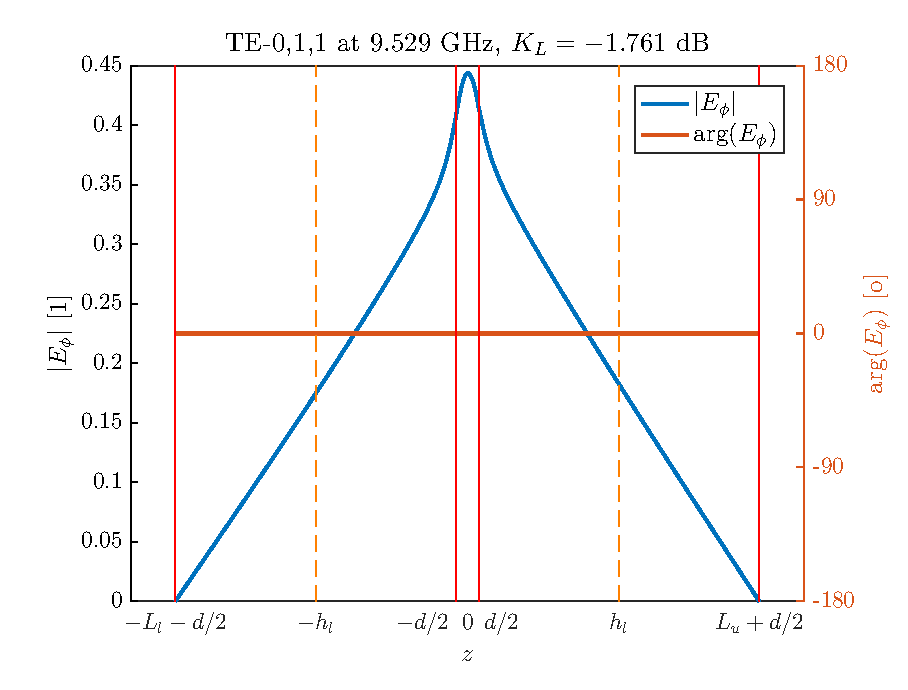
\includegraphics[width=0.8\textwidth]{mode_te011.eps}
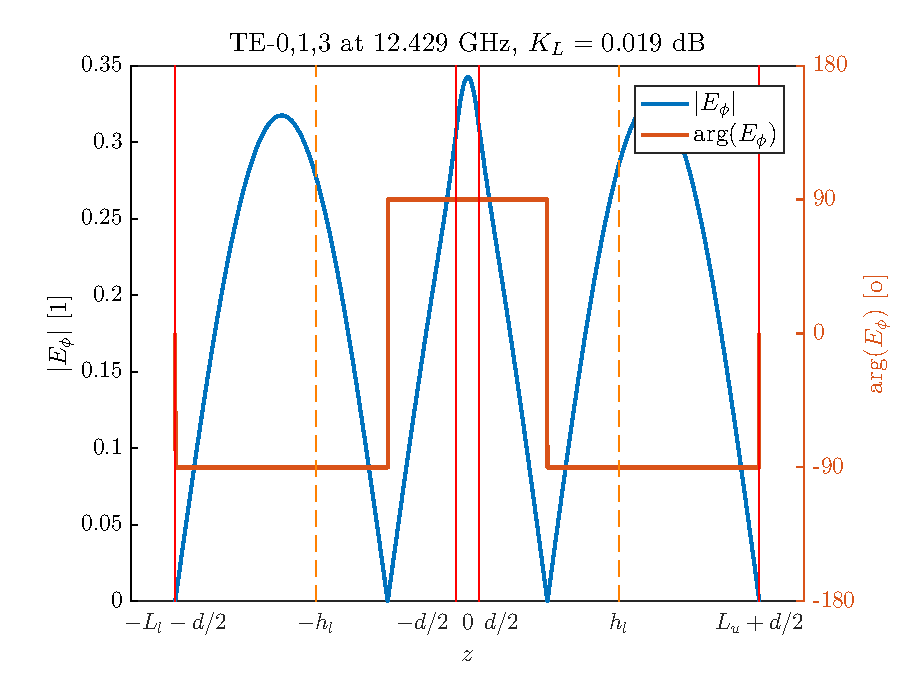
\includegraphics[width=0.8\textwidth]{mode_te013.eps}
\end{figure}

\begin{figure}
\centering
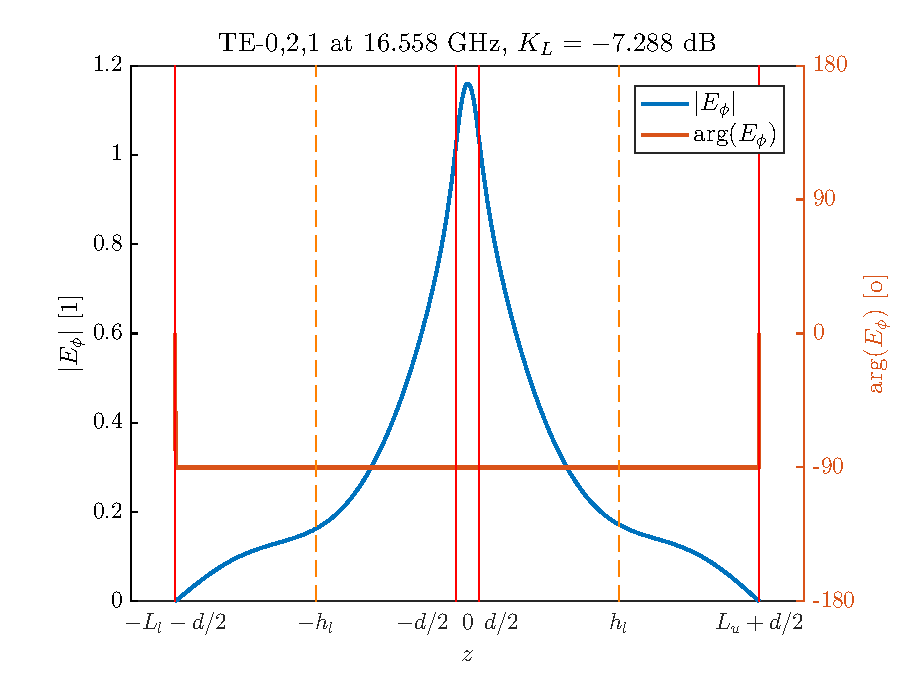
\includegraphics[width=0.8\textwidth]{mode_te021.eps}
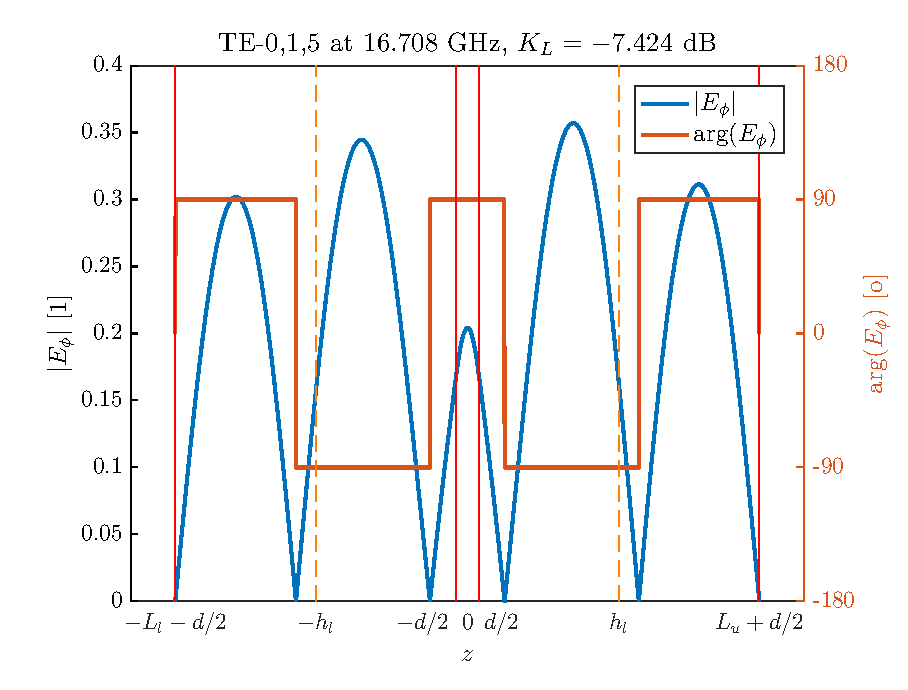
\includegraphics[width=0.8\textwidth]{mode_te015.eps}
\caption{The electric field $E_{\phi}(\rho=\frac{a_l}{2},z)$ of the first four odd TE\st{0np} modes of our split-cylinder resonator for a PTFE sample with a thickness of \SI{2}{\milli\meter}: The plot illustrates the absolute value and phase of the electric field of each mode along the z-axis. The relative permittivity of the sample $\epsilon_r$ is 2.056, the geometry of our resonator is used and 75 modes were included in the calculation. As a measure for the coupling of each mode a coupling constant $K_L=20\log(|H_{z,l}(\rho=a_l,z=h_l)|/\sqrt{4W_m/(V\mu_0)})$ is shown in the upper right corners of the plots.}\label{fig:first_modes}
\end{figure}

After this rather lengthy explanation of how to find and compute the modes of the split-cylinder resonator, we would like to include an example of a field calculation with our model to give the reader a useful insight into the method. It should also allow him to compare his implementation of the software to ours. As an example we computed the resonant frequencies of the first nine TE\st{0np} modes of our split-cylinder prototype for a PTFE sample. The sample had a thickness of \SI{2}{\milli\meter} and a relative permittivity $\epsilon_r$ of 2.056. We included 75 modes in the eigenmode expansion of the lower and upper cavity, as well as the right amount of modes in the specimen region to have optimum relative convergence. The nine modes included five odd TE\st{0np} modes, i.e. modes with an odd mode index $p$, and four even modes, i.e. modes with an even mode index $p$. Table \ref{tb:modes} lists the resonant frequencies and dominant modes of these first nine modes. Unlike Janezic's symmetric split-cylinder model, our asymmetric split-cylinder model also computes the even modes. These modes are in general not suitable for measurements, since the electric field vector of these modes has a minimum in the specimen region. This makes the fields of the modes less sensitive to the permittivity of the specimen and reduces the dielectric loss. While the former is less of a problem due to the high accuracy of our permittivity measurements, the latter reduces the accuracy of our dielectric measurements for low-loss dielectrics. Out of this reason, we usually also prefer the odd TE\st{0np} for complex permittivity measurements. In Fig. \ref{fig:first_modes} the electric field of the first four odd modes of our split-cylinder resonator for the PTFE sample is illustrated. As expected the electric field has a local maximum in the center of the substrate region. Apart from the electric field strength in the sample, Fig. \ref{fig:first_modes} also marks the location of the coupling loops in the cavity. Since the $z$ component of the magnetic field $H_z$ has the same minima along the z-axis as the electric field, the plot also illustrates the strength of the coupling of each mode.
\begin{table}
\centering
\begin{tabular}{|c|c|}
\hline\rule{0pt}{2.6ex}
Resonant frequency $f_r$ (\si{\giga\hertz}) & Mode \\
\hline\rule{0pt}{2.6ex}
 9.529 & TE\st{011} \\
11.178 & TE\st{012} \\
12.429 & TE\st{013} \\
14.970 & TE\st{014} \\
16.558 & TE\st{021} \\
16.708 & TE\st{015} \\
18.463 & TE\st{022} \\
18.959 & TE\st{023} \\
19.719 & TE\st{016} \\
\hline
\end{tabular}
\caption{Modes of our split-cylinder resonator from \SIrange{0.1}{20}{\giga\hertz} for a PTFE sample with a thickness of \SI{2}{\milli\meter}. The relative permittivity of the sample $\epsilon_r$ is 2.056, the geometry of our resonator is used and 75 modes were included in the calculation.}\label{tb:modes}
\end{table}
\section{Losses of the Measurement Model}\label{sec:losses}
As mentioned in the last chapter on the fields of the measurement model, the dielectric losses of the sample and the conductor losses of the cavity were neglected in the derivation of the field configuration of the resonator. It was acknowledged that these losses generally have a negligible influence on the fields in the cavity and that they can be neglected to simplify the field calculation. To measure the loss tangent $\tan\delta$ of a sample, which together with the dielectric constant $\epsilon$ constitutes the complex permittivity $\underline{\epsilon}=\epsilon-j\epsilon\tan\delta$, the losses must be reintroduced into our calculations. This is achieved as such that the field configuration in the resonator is computed with an $\epsilon_r$ measurement, where the measured $\epsilon_r$ is obtained from a measured resonant frequency $f_r$ and thickness $d$ of the sample, or from similar measurements. Then, the losses in the cavity are re-introduced by computing the dielectric loss
\begin{equation}\label{eq:d_loss}
P_d=\frac{1}{2}\iiint\limits_{\mathit{V}}\omega\epsilon\tan\delta\,|\vec{E}|^2\mathit{dV}\text{,}
\end{equation}
and the conductor losses
\begin{equation}\label{eq:c_loss}
P_c=\frac{R_s}{2}\iint\limits_{\mathit{A}}|\vec{H}_{t}|^2\mathit{dA}\text{,}
\end{equation}
where $R_s$ is the surface resistivity of the cavity, which we will obtain through a calibration, and $\vec{H}_{t}$ is the tangential magnetic field on the conductor surface \cite{pozar}.

The loss tangent is computed from the measured unloaded quality factor
\begin{equation}
Q_0=\omega\frac{\text{Stored energy}}{\text{Power dissipated}}=\left.\frac{\omega W}{P}\right\vert_{W(\omega_r)=2W_e(\omega_r)}=\frac{2\omega W_e}{P}\text{,}
\end{equation}
which is a ratio of the stored energy $W$ of a cavity and the power dissipated $P$ in a cavity. At resonance the magnetic energy is equal to electric energy in the cavity, so the total energy can be written as two times the electric energy of a cavity. The electric energy in the cavity is the volume integral of the squared magnitude of the electric field over the entire volume of the resonator,
\begin{equation}\label{eq:energy}
W_e=\iiint\limits_{\mathit{V}}\frac{1}{4}\epsilon|\vec{E}|^2\mathit{dV}\text{.}
\end{equation}

Broken down into the individual electric energies and losses the unloaded quality factor Q of the resonator is
\begin{equation}
Q_0=\frac{2\omega(W_u+W_s+W_l)}{P_{e,u}+P_{e,l}+P_{w,u}+P_{w,l}+P_{f,u}+P_{f,l}+P_s}\text{,}
\end{equation}
where $W_u$, $W_s$ and $W_l$ are the electric energies of the upper cavity region, sample region and lower cavity region. The losses of the resonator are divided into the conductor losses of the cavities and the dielectric loss of the sample $P_s$. The conductor losses are the losses on the surface of the metallic enclosure of the resonator, which we approximated as perfect electric conductors in our field derivation. These include the losses in the end plates, $P_{e,u}$ and $P_{e,l}$, in the walls, $P_{w,u}$ and $P_{w,l}$, and in the flanges, $P_{f,u}$ and $P_{f,l}$, of the upper and lower cavities, but naturally does not include the conductive boundary along the circumference of the sample that we introduced to approximate the split-cylinder with a closed cavity.

As the numerical integrals for the energies and losses are relatively computationally expensive, we can calculate the analytical integrals of the eigenmode expansions to simplify the computations. The volume integral of the squared magnitude of an electric field\eqref{eq:energy} gives us the electric energy in the upper cavity
\begin{align}
W_u =& \frac{\epsilon_{\text{lab}} }{4}\iiint\limits_{\mathit{V}}|\vec{E}|^2 \mathit{dV}=\frac{\epsilon_{\text{lab}}}{4}\int\limits_{\frac{d}{2}}^{\frac{d}{2}+L_u}\int\limits_0^{2\pi}\int\limits_0^{a_u} E_{\phi,u}E_{\phi,u}^* \rho\mathit{d\rho d\phi dz}\\
	=& \frac{\epsilon_{\text{lab}}\pi a_u^2}{4}\sum\limits_{n=1}^{N_u}|A_nU_nJ_0(h_{n,u}a_u)|^2\left\lbrace\frac{L_u}{2}-\frac{1}{4p_{n,u}}\sin(2p_{n,u}L_u)\right\rbrace\begin{cases}-1, &p_{n,u}\in\mathbb{I}\\1, &p_{n,u}\in\mathbb{R}\end{cases}\text{,}\label{eq:w_u}
 \end{align}
the electric energy in the sample region
\begin{align}
W_s =& \frac{\epsilon_r}{4}\iiint\limits_{\mathit{V}}|\vec{E}|^2 \mathit{dV}=\frac{\epsilon_r}{4}\int\limits_{-\frac{d}{2}}^{\frac{d}{2}}\int\limits_0^{2\pi}\int\limits_0^b E_{\phi,s}E_{\phi,s}^* \rho\mathit{d\rho d\phi dz}\\
	=& \frac{\epsilon_r\pi b^2}{4}\sum\limits_{m=1}^{N_s}J_0(h_{m,s}b)^2\times\nonumber\\&\begin{cases}|B_mV_m|^2(\frac{d}{2}+\frac{1}{2p_{m,s}}\sin(2p_{m,s}\frac{d}{2}))-|C_mW_m|^2(\frac{d}{2}-\frac{1}{2p_{m,s}}\sin(2p_{m,s}\frac{d}{2})), & p_{m,s}\in\mathbb{I}\\|B_mV_m|^2(\frac{d}{2}+\frac{1}{2p_{m,s}}\sin(2p_{m,s}\frac{d}{2}))+|C_mW_m|^2(\frac{d}{2}-\frac{1}{2p_{m,s}}\sin(2p_{m,s}\frac{d}{2})), & p_{m,s}\in\mathbb{R}\end{cases}
 \end{align}
 and the electric energy in the lower cavity
 \begin{align}
W_l =& \frac{\epsilon_{\text{lab}} }{4}\iiint\limits_{\mathit{V}}|\vec{E}|^2 \mathit{dV}=\frac{\epsilon_{\text{lab}}}{4}\int\limits_{-\frac{d}{2}-L_l}^{-\frac{d}{2}}\int\limits_0^{2\pi}\int\limits_0^{a_l} E_{\phi,l}E_{\phi,l}^* \rho\mathit{d\rho d\phi dz}\\
	=& \frac{\epsilon_{\text{lab}}\pi a_l^2}{4}\sum\limits_{p=1}^{N_l}|D_pL_pJ_0(h_{p,l}a_l)|^2\left\lbrace\frac{L_l}{2}-\frac{1}{4p_{p,l}}\sin(2p_{p,l}L_l)\right\rbrace\begin{cases}-1, &p_{p,l}\in\mathbb{I}\\1, &p_{p,l}\in\mathbb{R}\end{cases}\text{.}\label{eq:w_l}
 \end{align}
Similarly, the surface integral of the tangential magnetic field on the cavity surface \eqref{eq:c_loss} yields the losses of the upper cavity's end plate
\begin{align}
P_{e,u}=&\frac{R_s}{2}\iint\limits_{\mathit{A}}|\vec{H}_{t}|^2\mathit{dA}=\frac{R_s}{2}\int\limits_0^{2\pi}\int\limits_0^{a_u}H_{\rho,u}H_{\rho,u}^*\left(z=\frac{d}{2}+L_u\right) \rho\mathit{d\rho d\phi}\\ =& \frac{R_s\pi a_u^2}{\omega^2 \mu_0^2 2}\sum\limits_{n=1}^{N_u}|p_{n,u}A_nU_nJ_0(h_{n,u}a_u)|^2\text{,}\label{eq:p_eu}
\end{align}
the losses of the lower cavity's end plate
\begin{align}
P_{e,l}=&\frac{R_s}{2}\iint\limits_{\mathit{A}}|\vec{H}_{t}|^2\mathit{dA}=\frac{R_s}{2}\int\limits_0^{2\pi}\int\limits_0^{a_l}H_{\rho,l}H_{\rho,l}^*\left(z=-\frac{d}{2}-L_l\right) \rho\mathit{d\rho d\phi}\\ =& \frac{R_s\pi a_l^2}{\omega^2 \mu_0^2 2}\sum\limits_{p=1}^{N_l}|p_{p,l}D_pL_pJ_0(h_{p,l}a_l)|^2\text{,}\label{eq:p_el}
\end{align}
the losses in the walls of the upper cavity
\begin{align}
P_{w,u}=&\frac{R_s}{2}\iint\limits_\mathit{A}|\vec{H}_t|^2\mathit{dA}=\frac{R_s}{2}\int\limits_{\frac{d}{2}}^{\frac{d}{2}+L_u}\int\limits_0^{2\pi}H_{z,u}H_{z,u}^*(\rho=a_u)a_u\mathit{d\phi dz}\\
       =& \frac{R_s\pi a_u}{\omega^2\mu_0^2}\sum\limits_{n=1}^{N_u}\sum\limits_{n'=1}^{N_u}A_nA_{n'}^*U_nU_{n'}^*h_{n,u}h_{n',u}J_0(h_{n,u}a_u)J_0(h_{n',u}a_u)\times\nonumber\\&
       \begin{cases}
        	-\frac{1}{2}L_u+\frac{1}{4p_{n,u}}\sin(2p_{n,u}L_u), &(n=n') \wedge (p_{n,u}\in\mathbb{I})\\
        	 \frac{1}{2}L_u-\frac{1}{4p_{n,u}}\sin(2p_{n,u}L_u), &(n=n')  \wedge  (p_{n,u}\in\mathbb{R})\\
        	 \frac{\sin\left(\left(p_{n,u}-p_{n',u}\right)L_u\right)}{2\left(p_{n,u}-p_{n',u}^*\right)}-\frac{\sin\left(\left(p_{n,u}+p_{n',u}^*\right)L_u\right)}{2\left(p_{n,u}+p_{n',u}^*\right)}, &(n\neq n')
       \end{cases}\text{,}\label{eq:p_wu}
\end{align}
the losses in the walls of the lower cavity
\begin{align}
P_{w,l}=&\frac{R_s}{2}\iint\limits_\mathit{A}|\vec{H}_t|^2\mathit{dA}=\frac{R_s}{2}\int\limits_{-\frac{d}{2}-L_l}^{-\frac{d}{2}}\int\limits_0^{2\pi}H_{z,l}H_{z,l}^*(\rho=a_l)a_l\mathit{d\phi dz}\\
       =& \frac{R_s\pi a_l}{\omega^2\mu_0^2}\sum\limits_{p=1}^{N_l}\sum\limits_{p'=1}^{N_l}D_pD_{p'}^*L_pL_{p'}^*h_{p,l}h_{p',l}J_0(h_{p,l}a_l)J_0(h_{p',l}a_l)\times\nonumber\\&
       \begin{cases}
        	-\frac{1}{2}L_l+\frac{1}{4p_{p,l}}\sin(2p_{p,l}L_l), &(p=p') \wedge (p_{p,l}\in\mathbb{I})\\
        	 \frac{1}{2}L_l-\frac{1}{4p_{p,l}}\sin(2p_{p,l}L_l), &(p=p')  \wedge  (p_{p,l}\in\mathbb{R})\\
        	 \frac{\sin\left(\left(p_{p,l}-p_{p',l}\right)L_l\right)}{2\left(p_{p,l}-p_{p',l}^*\right)}-\frac{\sin\left(\left(p_{p,l}+p_{p',l}^*\right)L_l\right)}{2\left(p_{p,l}+p_{p',l}^*\right)}, &(p\neq p')
       \end{cases}\text{,}\label{eq:p_wl}
\end{align}
the losses on the flange of the upper cavity
\begin{align}
P_{f,u}=&\frac{R_s}{2}\iint\limits_\mathit{A}|\vec{H}_t|^2\mathit{dA}=\frac{R_s}{2}\int\limits_0^{2\pi}\int\limits_{a_u}^b H_{\rho,s}H_{\rho,s}^*\left(z=\frac{d}{2}\right)\rho \mathit{d\rho d\phi}\\
=& \frac{R_s\pi}{\omega^2\mu_0^2}\sum\limits_{m=1}^{N_s}\sum\limits_{m'=1}^{N_s}p_{m,s}p_{m',s}^* 
 \left\lbrace -B_mV_m\sin(p_{m,s}\frac{d}{2})+C_mW_m\cos(p_{m,s}\frac{d}{2})\right\rbrace\times\nonumber\\
 &\left\lbrace -B_{m'}V_{m'}\sin(p_{m',s}\frac{d}{2})+C_{m'}W_{m'}\cos(p_{m',s}\frac{d}{2})\right\rbrace^*\times\\\label{eq:p_fu}
 &\begin{cases}
 \frac{b^2}{2}J_0^2(h_{m,s}b)-\frac{a_u^2}{2}(J_0^2(h_{m,s}a_u)+J_1^2(h_{m,s}a_u))+\frac{a_u}{h_{m,s}}J_0(h_{m,s}a_u)J_1(h_{m,s}a_u),& m=m'\\
 -\frac{a_u}{h_{m,s}^2-h_{m',s}^2}(h_{m',s}J_1(h_{m,s}a_u)J_0(h_{m',s}a_u)-h_{m,s}J_0(h_{m,s}a_u)J_1(h_{m',s}a_u)),& m\neq m'
 \end{cases}\text{,}\nonumber
\end{align}
and the losses on the flange of the lower cavity
\begin{align}
P_{f,l}=&\frac{R_s}{2}\iint\limits_\mathit{A}|\vec{H}_t|^2\mathit{dA}=\frac{R_s}{2}\int\limits_0^{2\pi}\int\limits_{a_l}^b H_{\rho,s}H_{\rho,s}^*\left(z=-\frac{d}{2}\right)\rho \mathit{d\rho d\phi}\\
=& \frac{R_s\pi}{\omega^2\mu_0^2}\sum\limits_{m=1}^{N_s}\sum\limits_{m'=1}^{N_s}p_{m,s}p_{m',s}^* 
 \left\lbrace B_mV_m\sin(p_{m,s}\frac{d}{2})+C_mW_m\cos(p_{m,s}\frac{d}{2})\right\rbrace\times\nonumber\\
 &\left\lbrace B_{m'}V_{m'}\sin(p_{m',s}\frac{d}{2})+C_{m'}W_{m'}\cos(p_{m',s}\frac{d}{2})\right\rbrace^*\times\\
 &\begin{cases}
 \frac{b^2}{2}J_0^2(h_{m,s}b)-\frac{a_l^2}{2}(J_0^2(h_{m,s}a_l)+J_1^2(h_{m,s}a_l))+\frac{a_l}{h_{m,s}}J_0(h_{m,s}a_l)J_1(h_{m,s}a_l),& m=m'\\
 -\frac{a_l}{h_{m,s}^2-h_{m',s}^2}(h_{m',s}J_1(h_{m,s}a_l)J_0(h_{m',s}a_l)-h_{m,s}J_0(h_{m,s}a_l)J_1(h_{m',s}a_l)),& m\neq m'
 \end{cases}\text{.}\nonumber
\end{align}
Finally, the volume integral over the electric field \eqref{eq:d_loss} in the sample region leads to the dielectric loss of the sample
\begin{align}
P_s=&\frac{1}{2}\iiint\limits_{\mathit{V}}\omega\epsilon\tan\delta\,|\vec{E}|^2\mathit{dV}
   =\frac{\omega\epsilon'\tan\delta}{2}\int\limits_0^{2\pi}\int\limits_{-\frac{d}{2}}^{\frac{d}{2}}\int\limits_0^bE_{\phi,s}E_{\phi,s}^*\rho \mathit{d\rho dz d\phi}\nonumber\\
   =&\frac{\omega\epsilon_r\pi b^2\tan\delta}{2}\sum\limits_{m=1}^{N_s}J_0^2(h_{m,s}b)\times\\
   &\begin{cases}
   |B_mV_m|^2\left(\frac{d}{2}+\frac{1}{2p_{m,s}}\sin\left(2p_{m,s}\frac{d}{2}\right)\right)-|C_mW_m|^2\left(\frac{d}{2}-\frac{1}{2p_{m,s}}\sin\left(2p_{m,s}\frac{d}{2}\right)\right), & p_{m,s}\in \mathbb{I} \\
   |B_mV_m|^2\left(\frac{d}{2}+\frac{1}{2p_{m,s}}\sin\left(2p_{m,s}\frac{d}{2}\right)\right)+|C_mW_m|^2\left(\frac{d}{2}-\frac{1}{2p_{m,s}}\sin\left(2p_{m,s}\frac{d}{2}\right)\right), & p_{m,s}\in \mathbb{R}
   \end{cases}\text{.}\nonumber
\end{align}
The dielectric loss of the sample is proportional to the loss tangent $\tan\delta$. If we calculate the dielectric loss by subtracting the conductor losses from the total measured losses $P=\frac{2\omega W_e}{Q_0}$, we easily obtain the loss tangent
\begin{align}\label{eq:tand}
\tan\delta=\left(\frac{2\omega(W_u+W_s+W_l)}{Q_0}-P_{e,u}-P_{e,l}-P_{w,u}-P_{w,l}-P_{f,u}-P_{f,l}\right)/P_s'\text{,}
\end{align}
where $P_s'=P_s/\tan\delta$ is the normalised dielectric loss.
\subsection{Example of a Complex Permittivity Measurement Carried out with the M12 Model}\label{ss:ptfe}
Now that we have derived the entire M12 model we think the reader might benefit from an example of a complex permittivity measurement with the model. We only cover the calibration and the convergence of the model in the upcoming sections, so all the necessary theory is already available to us. In this example we are going to measure a PTFE sample with a thickness of \SI{1.509}{\milli\meter} with the TE\st{011} mode of the split-cylinder prototype. We begin with finding the TE\st{011} mode of the resonator: As we have already mentioned, the TE\st{011} mode is not the fundamental mode of the resonator and to complicate things even more the mode order in the split-cylinder depends on the dielectric constant of the specimen. Although coupling loops suppress the TM mode in the resonator, a number of TE modes still exist in the resonator making mode identification hard. An \er{} estimate is necessary to find the \te{} mode. This \er{} estimate may be a measurement with another method (e.g. a capacitance method), measurement data from a data sheet, or as suggested by Janezic \cite{janezicarz} an \er{} estimate from the fundamental TE\st{111} mode of the split-cylinder. It turns out that a simple split-cylinder model with a uniform diameter gives a reasonably accurate estimate of \er{}. We measured the transmission coefficient of the resonator of the fundamental mode (i.e. the first peak of the transmission coefficient) in the lab, which had its peak at \SI{5.2748}{\giga\hertz}. For this resonant frequency the model gives us an estimated \er{} of around 2.0815.
\begin{figure}
\centering
\begin{tikzpicture}
	\begin{axis}[	scale only axis,
					height=0.25\textheight,
					scaled x ticks=base 10:-9,
					xtick distance=0.05e9,
					xmin=9.53e9,
					xmax=9.774e9,
					xlabel={$f$ [\si{\hertz}]},
					ylabel={$20\log_{10}|S_{21}|$ [\si{\decibel}]},
					ymin=-100,
					ymax=-50]
		\addplot[blue] table[	col sep=comma,
								mark=none,
								x index=0,
								y index=1,
								header=false] {figures/PTFE_sample.csv};
		\node[pin=90:$TE_{011}$] at (9.6614e+09,-65.8523) {};		
	\end{axis}
\end{tikzpicture}
\caption{Resonance curve of the TE\st{011} mode of our split-cylinder prototype loaded with a \SI{1.509}{\milli\meter} thick PTFE sample. The resonant frequency of the mode was \SI{9.6619}{\giga\hertz} and the quality factor factor was \num{8754.3}, which both were obtained through a circle-fit of the resonance curve.}\label{fig:rc_ptfe}
\end{figure}

With this estimate for the dielectric constant \er{} we can now estimate the resonant frequency of the \te mode using the M12 model. For this we calculate the roots of the determinant 
\begin{equation}
\det(\mat{Z}(f,\epsilon_r=2.0815,d=\SI{1.509}{\milli\meter}))=0
\end{equation}
for the \er-estimate 2.0815 and the measured thickness of the sample $d=\SI{1.509}{\milli\meter}$. The first root at \SI{9.653}{\giga\hertz} is the estimated resonant frequency of the \te mode for the dielectric constant estimate and measured thickness. As the dielectric constant of low-dielectrics typically varies slowly with frequency the estimate should lie very closely to the true resonant frequency of the \te mode. Next, we need to measure the transmission coefficient around the resonant frequency estimate to find this true resonant frequency. Fig. \ref{fig:rc_ptfe} illustrates a measurement of the transmission coefficient that we performed around the estimate. To minimize the influence of the coupling network on this measurement we used very loose coupling. As there was only one resonance curve close to our estimate, the quality factor measurement of the curve gave us the resonant frequency \SI{9.6619}{\giga\hertz} and the quality factor \num{8754.3} of the \te mode. Our model allows us to compute the dielectric constant of our sample for this frequency by finding the first root of
\begin{equation}
\det(\mat{Z}(f=\SI{9.6619}{\giga\hertz},\epsilon_r,d=\SI{1.509}{\milli\meter}))=0\text{.}
\end{equation}
The first root and the dielectric constant of the sample is $\epsilon_r=2.0563$, for which the field configuration is shown in Fig. \ref{fig:mode_ptfe}. Lastly, we can use the solution of this measurement to calculate the \tand{} with Equation \eqref{eq:tand} from the surface resistance $R_s$ of the resonator and the measured quality factor $Q$ of the mode. The result of the equation is the loss tangent $\tan\delta=\num{2.2208e-4}$.
\begin{figure}
\centering
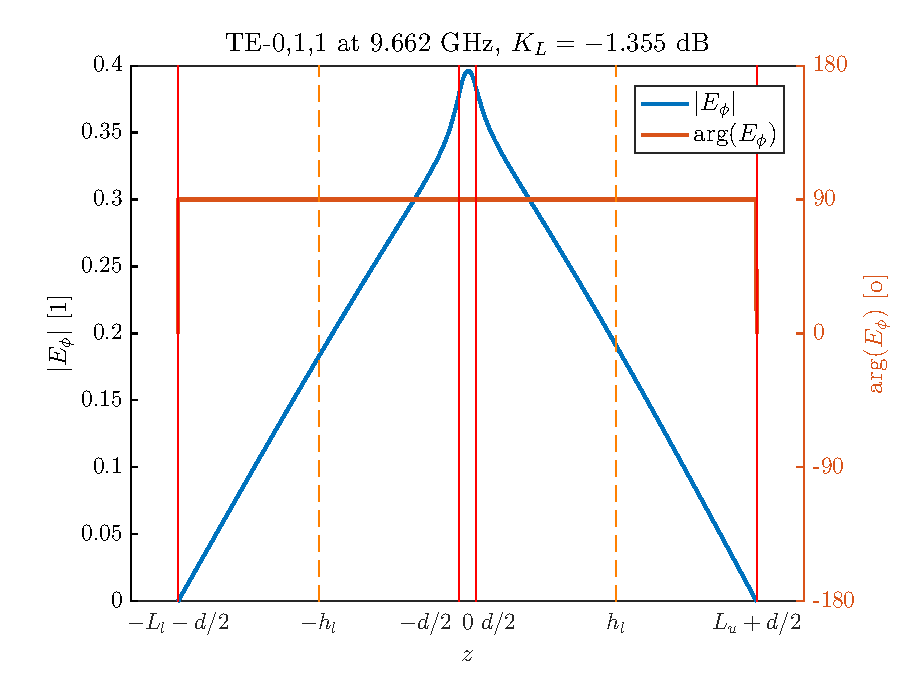
\includegraphics[height=0.3\textheight]{PTFE_sample.eps}
\caption{The electric field $E_{\phi}(\rho=\frac{a_l}{2},z)$ of the TE\st{011} mode of the sample along the z-axis of the split-cylinder. The sample was a \SI{1.509}{\milli\meter} thick PTFE sample with a dielectric constant $\epsilon$ of \num{2.0563}. The plot also indicates the boundaries of the resonator and the location of the coupling loops. As a measure for the coupling of the mode a coupling constant $K_L$ is shown in the upper right corner of the plot.}\label{fig:mode_ptfe}
\end{figure}
\section{Fields of the Calibration Model}
\begin{figure}
\centering
\begin{tikzpicture}
   %\draw[step=1cm,gray,very thin] (0,0) grid (8,7);
    \node[anchor=south west,inner sep=0] (image) at (0,0) {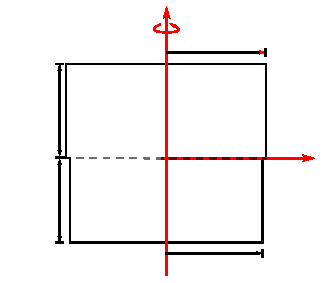
\includegraphics[width=8cm]{split_cylinder_resonator_cal_model.pdf}};
    \draw (4,6.9) node[red] {\textit{z}};
    \draw (7.75,3) node[red] {\textit{$\rho$}};
    \draw (1,4.1) node {$L_u$};
    \draw (1,2) node {$L_l$};
    \draw (5.2,5.85) node {$a_u$};
    \draw (5.2,0.4) node {$a_l$};
    
    \draw (2.4,2) node[anchor=west] {\scalebox{0.75}{$\mu_0,\epsilon_{lab}$}};
    \draw (2.4,4.10) node[anchor=west]  {\scalebox{0.75}{$\mu_0,\epsilon_{lab}$}};
\end{tikzpicture}
\caption{Geometry of the asymmetric split-cylinder's calibration model.}\label{fig:cal_model}
\end{figure}
In the previous sections we have taken a closer look at the M12 model, which we developed and tested during the course of these sections. We also recognised that the M12 model used a large number of variables to compute the modes of the resonator and that therefore the accuracy of the model relied on the accuracy of these variables. Like for any physical model the actual measurement variables and the setup of the resonator must closely resemble the measurement variables and the geometry of the model. Unfortunately, this model has a few systematic errors that are not part of the model and that disturb our measurements. During our measurements we identified a few potential sources of systematic error, which include:
\begin{itemize}
\item Geometry of the cavities (Taper of the cylindrical cavities, parallelism and flatness of the cylinder faces, ...)
\item Properties of the setup (Eccentricity of the two half-cylinders, unequal surface losses due to surface finish variations, dust and dirt)
\item Properties of the sample (Compression of the sample, geometry of the sample (flatness, parallelism), impurities)
\end{itemize}
Although these systematic errors cannot be avoided altogether, there are strategies to minimise these uncertainties. One strategy is an error correction based on a calibration. In such a strategy a calibration standard is measured and using a reference value for the calibration standard the measurement model is adjusted to zero out the difference between the measured value and the reference value. Janezic \cite{janezic} included a calibration procedure in his split-cylinder model that involved a measurement of the empty split-cylinder resonator. In this procedure the dielectric sample is removed from the resonator and both half-cavities are pressed together without a sample in between. The symmetric split-cylinder is turned into a cylindrical cavity! Then, the resonance curve of the TE\st{011} mode is measured and the result of the measurement is used to adjust the radius $a$ and the conductivity $\sigma$ of resonator. While both compensate for the systematic errors in the measurement, the radius $a$ predominantly compensates for variations in the geometry of the setup and the conductivity $\sigma$ for the variations in the surface finish. With the conductivity $\sigma$ of the calibration we also obtain the surface resistance $R_s$ of the resonator, which is a necessary variable for the calculation of the loss tangent $\tan\delta$. This is a very important parameter of the calibration as the surface conductivity differs largely from the bulk conductivity. The surface conductivity also depends on parameters like surface roughness or contaminants, which can reduce the conductivity by more than \SI{50}{\percent} compared to the bulk conductivity. This makes the calibration of the conductivity $\sigma$ absolutely vital to accurate loss tangent measurements.

As the M12 model is based on Janezic's mode-matching model, we also decided to use a calibration for the M12 model. Like in Janezic's model the resonator is calibrated by pressing the two half-cavities together. This makes an asymmetric closed cavity out of our asymmetric split cylinder, which is not a cylindrical cavity like in Janezic's model. Out of this reason we developed a second mode-matching model exclusively for the calibration, which uses the radius of the lower cavity $a_l$ and the conductivity $\sigma$ as calibrations parameters. Even though our model uses the same calibration as Janezic's, we added a broadband calibration feature to our model. While Janezic's model only used the TE\st{011} mode for its calibration, we decided to use all available modes in our calibration. We recognised that the systematic errors of the measurements varied with each mode and that the calibration for another mode gave different results for the parameters $a_l$ and $\sigma$. We assumed that this behaviour was due to fact that the different field configurations of the modes emphasize different systematic errors. The conductivity of the resonator, for example, may vary with the different distributions of the magnetic fields on the surface of the cavity, since a lossy surface can lie in a region with high field strength for one mode and can lie in a low point for another. In our measurements we observed that the broadband calibration generally improved the measurement accuracy of higher TE\st{0np} modes of the resonator.

The derivation of our calibration model is very similar to the derivation of the M12 model. This is not very surprising, since the boundary value problem is identical to the original model, if we let the thickness of the sample become zero $d\rightarrow 0$. Although the boundary value problem is identical, we still need to match the modes at the new interface to find a solution. To do this we first take the solutions of the boundary value problem of the cylindrical waveguide of the upper cavity \eqref{eq:e_u}\eqref{eq:h_u}
\begin{align}
E_{\phi,u}(\rho,z)&=\sum\limits_{n=1}^{\infty} A_nU_nJ_1(h_{n,u}\rho)\sin(p_{n,u}\left(L_u-z\right)), &\scriptstyle (0\leq\rho\leq a_u)\wedge\left(0\leq z\leq L_u\right)\label{eq:e_uc}\\
H_{\rho,u}(\rho,z)&=\sum\limits_{n=1}^{\infty}\frac{-p_{n,u}}{j\omega\mu_0}A_nU_nJ_1(h_{nu}\rho)\cos(p_{n,u}\left(L_u-z\right)),&\scriptstyle\left(0\leq\rho\leq  a_u\right)\wedge\left(0\leq z\leq L_u\right)\label{eq:h_uc}\\
H_{z,u}(\rho,z)&=\frac{-1}{j\omega\mu_0}\sum\limits_{n=1}^\infty A_nU_nh_{n,u}J_0(h_{n,u}\rho)\sin(p_{n,u}\left(L_u-z\right)),&\scriptstyle(0\leq\rho\leq a_u)\wedge\left(0\leq z\leq L_u\right)
\end{align}
and the lower cavity \eqref{eq:e_l}\eqref{eq:h_l}
\begin{align}
E_{\phi,l}(\rho,z)&=\sum\limits_{p=1}^{\infty} D_pL_pJ_1(h_{p,l}\rho)\sin(p_{p,l}\left(z+L_l\right)), & \scriptstyle(0\leq\rho\leq a_l)\wedge\left(-L_l\leq z\leq 0\right)\label{eq:e_lc}\\
H_{\rho,l}(\rho,z)&=\sum\limits_{p=1}^{\infty}\frac{p_{p,l}}{j\omega\mu_0}D_pL_pJ_1(h_{p,l}\rho)\cos(p_{p,l}\left(z+L_l\right)), &\scriptstyle(0\leq\rho\leq a_l)\wedge\left(-L_l\leq z\leq 0\right)\label{eq:h_lc}\\
H_{z,l}(\rho,z)&=\frac{-1}{j\omega\mu_0}\sum\limits_{p=1}^\infty D_pL_ph_{p,l}J_0(h_{p,l}\rho)\sin(p_{p,l}\left(z+L_l\right)), &\scriptstyle(0\leq\rho\leq a_l)\wedge\left(-L_l\leq z\leq 0\right)\text{.}
\end{align}
As can be seen in Fig. \ref{fig:cal_model}, we only have one interface at $z=0$ in this boundary value problem, where need to match the eigenmode expansions of the fields in the cavity. Like for the M12 model, the mode matching at the interface solves the boundary value problem of the TE\st{0np} modes. The first boundary condition is the continuity of the tangential electric field
\begin{align}\label{eq:bcc_1}
E_{\phi,u}\left(\rho,z=0\right)= \begin{cases}
    E_{\phi,l}(\rho,z=0) , & 0\leq\rho\leq a_l\\
    0, & a_l\leq\rho\leq a_u
  \end{cases}\text{,}
\end{align}
which matches the electric field of the upper cavity to that of the lower cavity at the interface. Like in the previous derivations, we again insert the fields \eqref{eq:e_uc}\eqref{eq:e_lc} into the boundary condition and compute the scalar product of the tangential electric field and $H_{\rho,u}^{(n)}$ on each side of the equation. Since only the first-order Bessel function of the first kind $J_1(h_{n,u}\rho)$ of $H_{\rho,u}^{(n)}$ varies with $\rho$, we can compute
\begin{equation}
\begin{split}
\int\limits_0^{2\pi}\int\limits_0^{a_u}\sum\limits_{n'=1}^\infty A_{n'}U_{n'}J_1(h_{n',u}\rho)\sin(p_{n',u}L_u)J_1(h_{n,u}\rho)\rho\mathit{d\rho d\phi}\\=\int\limits_0^{2\pi}\int\limits_0^{a_l}\sum\limits_{p=1}^\infty D_{p}L_{p}J_1(h_{p,l}\rho)\sin(p_{p,l}L_l)J_1(h_{n,u}\rho)\rho\mathit{d\rho d\phi}
\end{split}\text{.}
\end{equation}
With help from the orthogonality relation of \eqref{eq:o_u}, we can compute the result of the integral, the mode-matching equation of the electric field
\begin{equation}\label{eq:c_mm_e}
A_nU_n\sin(p_{n,u}L_u)\frac{a_u^2}{2}J_0^2(h_{n,u}a_u)=\sum\limits_{p=1}^\infty D_pL_p\sin(p_{p,l}L_l)\frac{-h_{p,l}a_l}{h_{p,l}^2-h_{n,u}^2}J_0(h_{p,l}a_l)J_1(h_{n,u}a_l)\text{.}
\end{equation}

The second boundary condition is the continuity of the tangential magnetic field \eqref{eq:bcc_2} at the interface. We demand that the $\rho$ component of the magnetic field must be continuous over the entire surface of the boundary at $z=0$.
\begin{equation}\label{eq:bcc_2}
H_{\rho,u}\left(\rho,z=0\right)= H_{\rho,l}\left(\rho,z=0\right),\qquad 0\leq\rho\leq a_l
\end{equation}
Again, we enforce the boundary condition by matching the modes at the interface. Hence, we insert the eigenmode expansions of the magnetic fields \eqref{eq:h_uc}\eqref{eq:h_lc} into the boundary condition and calculate the scalar product of the tangential magnetic fields and $E_{\phi,l}^{(p)}$. This scalar product is an integral of the product of the expansion and the mode $E_{\phi,l}^{(p)}$ over the surface of the boundary
\begin{equation}
\begin{split}
\int\limits_0^{2\pi}\int\limits_0^{a_l}\sum\limits_{n=1}^\infty \frac{-p_{n,u}}{j\omega\mu_0}A_{n}U_{n}J_1(h_{n,u}\rho)\cos(p_{n,u}L_u)J_1(h_{p,l}\rho)\rho\mathit{d\rho d\phi}\\=\int\limits_0^{2\pi}\int\limits_0^{a_l}\sum\limits_{p'=1}^\infty \frac{p_{p',l}}{j\omega\mu_0}D_{p'}L_{p'}J_1(h_{p',l}\rho)\cos(p_{p',l}L_l)J_1(h_{p,l}\rho)\rho\mathit{d\rho d\phi}
\end{split}\text{,}
\end{equation}
where we once more use the Bessel function instead of the whole field. If we employ the orthogonality relation of the lower cavity \eqref{eq:o_l}, the result is the mode-matching equation of the magnetic field
\begin{equation}\label{eq:c_mm_h}
\sum\limits_{n=1}^\infty A_nU_n\frac{a_lh_{p,l}p_{n,u}}{h_{p,l}^2-h_{n,u}^2}J_0(h_{p,l}a_l)J_1(h_{n,u}a_l)\cos(p_{n,u}L_u)=D_pL_p\frac{a_l^2}{2}p_{p,l}J_0^2(h_{p,l}a_l)\cos(p_{p,l}L_l)\text{.}
\end{equation}
With the two mode-matching equations at hand we can now solve the boundary value problem of the calibration. If we limit the number of modes of the eigen-mode expansions of the mode-matching equations \eqref{eq:c_mm_e} and \eqref{eq:c_mm_h} to $N_u$ modes for the upper cavity and $N_l$ modes for the lower cavity, each infinite series of the mode-matching equations becomes a finite series. Since we calculated the mode-matching equations as a scalar product of the expansion with a single mode from the upper cavity or the lower cavity, we actually get $N_s+N_l$ equations out of the two mode-matching equations. With this number of equations and the same number of unknowns the equations become a uniquely determined homogeneous system of linear equations, which we can easily solve. To simplify the notation, we can write the homogeneous system of linear equations as the matrix equation
\begin{equation}\label{eq:matZc}
\mat{Z}\vec{x}=\mat{Z}\begin{bmatrix}\vec{A}\\\vec{D}\\\end{bmatrix}=
\begin{bmatrix}
\mat{C_1}&-\mat{C_2}\\
\mat{C_3}&-\mat{C_4}\\
\end{bmatrix}\begin{bmatrix}\vec{A}\\\vec{D}\\\end{bmatrix}=
\vec{0}\text{,}
\end{equation}
where $\mat{Z}$ is the mode-matching matrix and $\vec{x}$ is a coefficient vector that contains the coefficients of the eigenmode expansion $A_n$ and $D_p$. The matrix $\mat{Z}$ contains all the equations of the mode-matching problem, which are grouped in sub-matrices $\mat{C_1}$, $\mat{C_2}$, $\mat{C_3}$ and $\mat{C_4}$. Apparently, any solution $\vec{x}$ of the matrix equation is a solution of the boundary value problem.
\begin{align}
(\mat{C_1})_{nn}&= U_n\sin(p_{n,u}L_u)\frac{a_u^2}{2}J_0^2(h_{n,u}a_u)\\
(\mat{C_2})_{np}&= L_p\sin(p_{p,l}L_l)\frac{-h_{p,l}a_l}{h_{p,l}^2-h_{n,u}^2}J_0(h_{p,l}a_l)J_1(h_{n,u}a_l)\\
(\mat{C_3})_{pn}&= U_n\frac{a_lh_{p,l}p_{n,u}}{h_{p,l}^2-h_{n,u}^2}J_0(h_{p,l}a_l)J_1(h_{n,u}a_l)\cos(p_{n,u}L_u)\\
(\mat{C_4})_{pp}&= L_p\frac{a_l^2}{2}p_{p,l}J_0^2(h_{p,l}a_l)\cos(p_{p,l}L_l)
\end{align}
Analogous to the M12 matrix, a singular matrix $\mat{Z}$ is a necessary condition for the existence of a solution of Equation \eqref{eq:matZc}. Owing to this fact, root-finding algorithms can be used to find roots of the determinant of the matrix
\begin{equation}
\det(\mat{Z}(f=f_r,a_l))=0\text{,}
\end{equation}
which for each mode used in our calibration gives a lower cavity radius $a_l$. Eventually, each lower cavity radius $a_l$ can be used a calibration parameter for the mode it was calibrated with.
\section{Losses of the Calibration Model}
The loss mechanisms of the calibration are to a large extent identical to that of the original model. We will therefore abbreviate the derivation and we will not include the integrals of the electric energy and the conductor losses, which all can be found in Section \ref{sec:losses}. The unloaded quality factor $Q_0$ is again the ratio of the electric energy to the losses in the cavity
\begin{align}
Q_0 =& \frac{2\omega(W_u+W_l)}{P_{e,u}+P_{e,l}+P_{w,u}+P_{w,l}+P_{f,u}}\\=&\frac{2\omega(W_u+W_l)}{R_s(P'_{e,u}+P'_{e,l}+P'_{w,u}+P'_{w,l}+P'_{f,u})} = \frac{2\omega(W_u+W_l)}{R_sP'}\text{,}
\end{align}
where $W_u$ and $W_l$ are the electric energy in the cavities, $P_{e,u}$ and $P_{e,l}$ are the losses in the end plates, $P_{w,u}$ and $P_{w,l}$ are the losses in the walls of the cavities, and $P_{f,l}$ is the flange loss at the interface between the two cavities. As all losses in the cavity are conductor loss we can normalize the losses and write the total loss in the cavity as the normalized loss $P'$ multiplied with the surface resistance $R_s$. Although the electric energies and losses are very similar to the ones of the M12 model, we find that it would be useful for the reader to at least list them here. The electric energy of the upper cavity was already calculated by us in \eqref{eq:w_u}
\begin{align}
W_u =& \frac{\epsilon_{\text{lab}}\pi a_u^2}{4}\sum\limits_{n=1}^{N_u}|A_nU_nJ_0(h_{n,u}a_u)|^2\left\lbrace\frac{L_u}{2}-\frac{1}{4p_{n,u}}\sin(2p_{n,u}L_u)\right\rbrace\begin{cases}-1, &p_{n,u}\in\mathbb{I}\\1, &p_{n,u}\in\mathbb{R}\end{cases}\text{,}
 \end{align}
and the electric energy of the lower cavity was calculated in \eqref{eq:w_l}
  \begin{align}
W_l =& \frac{\epsilon_{\text{lab}}\pi a_l^2}{4}\sum\limits_{p=1}^{N_l}|D_pL_pJ_0(h_{p,l}a_l)|^2\left\lbrace\frac{L_l}{2}-\frac{1}{4p_{p,l}}\sin(2p_{p,l}L_l)\right\rbrace\begin{cases}-1, &p_{p,l}\in\mathbb{I}\\1, &p_{p,l}\in\mathbb{R}\end{cases}\text{.}
 \end{align}
For the conductor losses we use our results for the losses of the upper cavity's end plate
\begin{align}
P_{e,u}=& \frac{R_s\pi a_u^2}{\omega^2 \mu_0^2 2}\sum\limits_{n=1}^{N_u}|p_{n,u}A_nU_nJ_0(h_{n,u}a_u)|^2
\end{align}
given in Equation \eqref{eq:p_eu} and the results for the losses of the lower cavity's end plate
\begin{align}
P_{e,l}=& \frac{R_s\pi a_l^2}{\omega^2 \mu_0^2 2}\sum\limits_{p=1}^{N_l}|p_{p,l}D_pL_pJ_0(h_{p,l}a_l)|^2
\end{align}
given in Equation \eqref{eq:p_el}. Next, we use our calculations of the losses in the upper cavity walls $P_{w,u}$ shown in Eq. \eqref{eq:p_wu} 
\begin{align}
P_{w,u}=& \frac{R_s\pi a_u}{\omega^2\mu_0^2}\sum\limits_{n=1}^{N_u}\sum\limits_{n'=1}^{N_u}A_nA_{n'}^*U_nU_{n'}^*h_{n,u}h_{n',u}J_0(h_{n,u}a_u)J_0(h_{n',u}a_u)\times\nonumber\\&
       \begin{cases}
        	-\frac{1}{2}L_u+\frac{1}{4p_{n,u}}\sin(2p_{n,u}L_u), &(n=n') \wedge (p_{n,u}\in\mathbb{I})\\
        	 \frac{1}{2}L_u-\frac{1}{4p_{n,u}}\sin(2p_{n,u}L_u), &(n=n')  \wedge  (p_{n,u}\in\mathbb{R})\\
        	 \frac{\sin\left(\left(p_{n,u}-p_{n',u}\right)L_u\right)}{2\left(p_{n,u}-p_{n',u}^*\right)}-\frac{\sin\left(\left(p_{n,u}+p_{n',u}^*\right)L_u\right)}{2\left(p_{n,u}+p_{n',u}^*\right)}, &(n\neq n')
       \end{cases}
\end{align}
and those of the losses in the lower cavity walls $P_{w,l}$ shown Eq. \eqref{eq:p_wl} 
\begin{align}
P_{w,l}=& \frac{R_s\pi a_l}{\omega^2\mu_0^2}\sum\limits_{p=1}^{N_l}\sum\limits_{p'=1}^{N_l}D_pD_{p'}^*L_pL_{p'}^*h_{p,l}h_{p',l}J_0(h_{p,l}a_l)J_0(h_{p',l}a_l)\times\nonumber\\&
       \begin{cases}
        	-\frac{1}{2}L_l+\frac{1}{4p_{p,l}}\sin(2p_{p,l}L_l), &(p=p') \wedge (p_{p,l}\in\mathbb{I})\\
        	 \frac{1}{2}L_l-\frac{1}{4p_{p,l}}\sin(2p_{p,l}L_l), &(p=p')  \wedge  (p_{p,l}\in\mathbb{R})\\
        	 \frac{\sin\left(\left(p_{p,l}-p_{p',l}\right)L_l\right)}{2\left(p_{p,l}-p_{p',l}^*\right)}-\frac{\sin\left(\left(p_{p,l}+p_{p',l}^*\right)L_l\right)}{2\left(p_{p,l}+p_{p',l}^*\right)}, &(p\neq p')
       \end{cases}\text{.}
\end{align}
Finally, the only remaining loss is the flange loss at the interface, which is similar to the flange loss we calculated in Eq. \eqref{eq:p_fu}.
\begin{align}
P_{f,u}=& \frac{R_s\pi}{\omega^2\mu_0^2}\sum\limits_{n=1}^{N_s}\sum\limits_{n'=1}^{N_s}p_{n,u}p_{n',u}^*A_nA_{n'}^*U_nU_{n'}^*\cos(p_{n,u}L_u)\cos(p_{n',u}L_u)^*\times\\
 &\begin{cases}
 \frac{a_u^2}{2}J_0^2(h_{n,u}a_u)-\frac{a_l^2}{2}(J_0^2(h_{n,u}a_l)+J_1^2(h_{n,u}a_l))+\frac{a_l}{h_{n,u}}J_0(h_{n,u}a_l)J_1(h_{n,u}a_l),& n=n'\\
 -\frac{a_l}{h_{n,u}^2-h_{n',u}^2}(h_{n',u}J_1(h_{n,u}a_l)J_0(h_{n',u}a_l)-h_{n,u}J_0(h_{n,u}a_l)J_1(h_{n',u}a_l)),& n\neq n'
 \end{cases}\text{,}\nonumber
\end{align}
We can then use the results for the electric energies and the conductor losses to compute the conductivity of the cavity
\begin{equation}
\sigma = \frac{\omega\mu_0}{2R_s^2}=\frac{\omega\mu_0}{2}\left(\frac{2\omega(W_u+W_l)}{Q_0P'}\right)^{-2}\text{.}
\end{equation}
This conductivity $\sigma$ is the second parameter of our calibration and allows us to calibrate the cavity for accurate loss tangent $\tan\delta$ measurements. Like the first parameter of the calibration, the lower cavity radius $a_l$, the conductivity can be calibrated not only with the TE\st{011} mode, but with multiple modes. This allows us to use different conductivities for different modes and improve the accuracy of loss tangent measurements with higher modes.
\section{Convergence of Both Models}
After we have derived both the M12 model and the calibration model for the M12 model, we still have to discuss the convergence of these mode-matching models. Although mode-matching has properties of an analytical technique, it is a numerical method and it is therefore supposed to converge to a true value with increasing numerical accuracy. We have already mentioned that mode-matching achieves this by matching the boundary condition at the interface between two field regions. In these field regions the electro-magnetic field is expanded as an infinitely long series and the mode-matching method gives an mathematically exact solution only for these infinitely long series. An exact solution is identical to a perfect match of the boundary conditions and a solution of the boundary-value problem. As an infinitely long series cannot be computed on a computer, the infinite series are truncated after a few terms and the truncated series are used to approximate the exact solution. While it is somewhat logical that the truncation of the series introduces a numerical error, a reduction of the numerical error with increasing numerical accuracy, i.e. the convergence of the mode-matching model, cannot be expected for every truncated series. It turns out that a mode-matching calculation can converge to different results depending on the number of modes used for the expansion in each region. More specifically, if the number of modes are increased equally in the regions, the result does not have to converge or converges very slowly. This phenomenon is called relative convergence and has been studied by many researchers \cite{itoh, mittra, leroy, sorrentino}. Although we could find a conclusive explanation of the phenomenon, the edge effect at boundaries \cite{mittra} and ill-conditioned equation systems \cite{leroy} were identified by others as root causes of the phenomenon. Another explanation suggested that fluctuations of one field must be supported by the modes in the other, so that the spectral content on both sides is the same.

\begin{figure}
\centering
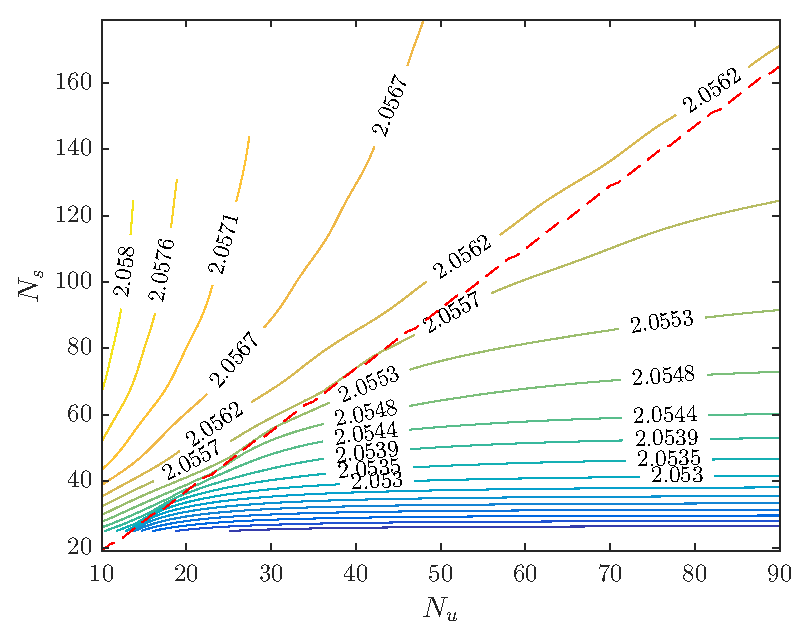
\includegraphics[scale=0.75]{RC_er.eps}
\caption{Contour plot of the relative permittivity of the PTFE sample. The permittivity is plotted against the number of modes of the sample region $N_s$ and against that of the upper cavity $N_u$. The resonant frequency used for the plot was \SI{9.6619}{\giga\hertz} and the thickness of the sample was \SI{1.509}{\milli\meter}. The dashed line shows the ideal model ratio of $N_s$ and $N_u$ according to Il'inksi \cite{ilinski} and Janezic \cite{janezic}.}\label{fig:RCer}
\end{figure}

Irrespective of the origins of the relative convergence, the relative convergence should be minimised to ensure fast convergence and low computational effort. On the one hand Janezic \cite{janezic} noted that this can be achieved by employing all available orthogonality relations. On the other hand an optimum mode ratio must be chosen for the expansions, which is the ratio of the number of modes of one region to that of another region that gives the best convergence for the computational effort spent. Different optimum mode ratios for the mode-matching method can be found in the literature. Janezic suggested with reference to an article by Il'inski \cite{ilinski} that the propagation constant $p_N$ of the highest expansion mode in each section must be equal. Earlier research used ratios of the lateral extension of two guides, but then again others found that the ratio must be chosen as such that the cut-off wave number $h_N$  is the same in each guide. As the cut-off wave number of higher modes is typically far higher than the wave number $k$, these three optimum mode ratios yield the same results for higher modes. 

\begin{figure}
\centering
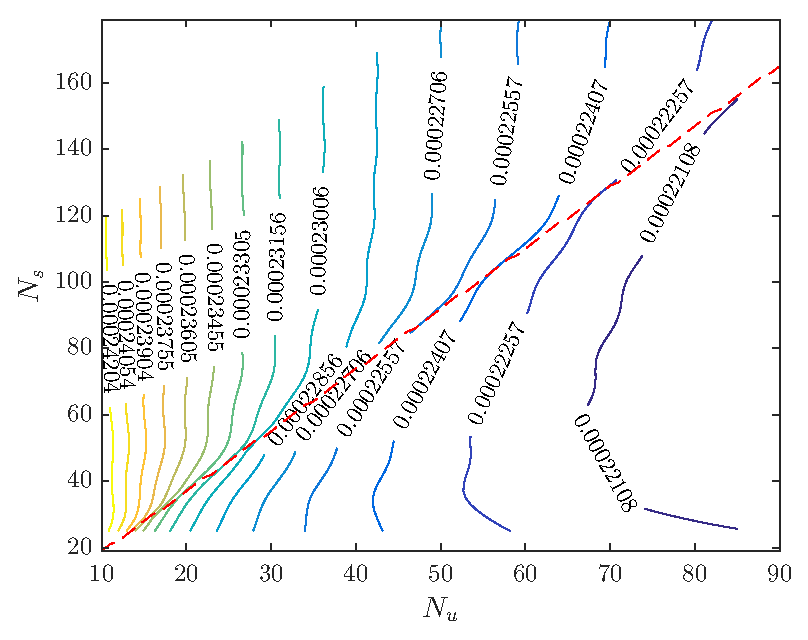
\includegraphics[scale=0.75]{RC_tand.eps}
\caption{Contour plot of the loss tangent of the PTFE sample. The loss tangent is plotted against the number of modes of the sample region $N_s$ and against that of the upper cavity $N_u$. The resonant frequency used for the plot was \SI{9.6619}{\giga\hertz}, the unloaded quality factor $Q_0$ of the resonance was \num{8754.3} and the thickness of the sample was \SI{1.509}{\milli\meter}. The dashed line shows the ideal model ratio of $N_s$ and $N_u$ according to Il'inksi \cite{ilinski} and Janezic \cite{janezic}.}\label{fig:RCtand}
\end{figure}

For the derivation of the M12 model and for that of the calibration model we naturally used all available orthogonality relations, and for our computations we also used the optimum mode ratios. To illustrate the relative convergence of the model we can plot the relative permittivity against the number of modes in the sample region and against that in the upper cavity. Again, we use the same PTFE sample that we used for most of our examples up to now, for which we measured a resonant frequency of \SI{9.6619}{\giga\hertz}, an unloaded quality factor \num{8754.3} and a thickness of \SI{1.509}{\milli\meter}. As can be seen in Fig. \ref{fig:RCer}, the convergence of the relative permittivity indeed varies with the number of modes. We also added a plot of Il'inski's optimum mode ratio to show how a mode matching model converges for an optimum mode ratio, which is marked by a dashed line in the plot. The plot exemplifies that the model converges optimally for the optimum mode ratio and that the result converges rapidly when we increase the number of modes in this ratio. It also shows that the convergence error for this ratio becomes less than \num{5e-4} for only $N_u=50$ modes. As can be seen in Fig. \ref{fig:RCtand} the relative convergence phenomenon has an influence on the loss tangent as well. As the accuracy of our loss tangent measurements is typically lower, the influence of the relative convergence on the loss tangent is less pronounced. Since our model was designed with split-cylinders in mind that have only a small difference in the geometry of their cavities, we chose $N_u=N_l$ for the computation of these plots. If we use the Il'inski optimum mode ratio for both interfaces
\begin{align}
p_{N_u,u}=p_{N_s,s} \quad\quad\quad p_{N_s,s}=p_{N_l,l}
\end{align} 
this small difference also makes $N_u$ and $N_l$ become approximately equal, $N_u\approx N_l$. For the calibration model the situation is very similar, since the variables that define the propagation constants, i.e. relative permittivity of the air in the cavities and the radii of the cavities, are equal or almost equal. Accordingly, optimum convergence of the calibration model can be achieved with the mode ratio $N_u=N_l$. Since the ideal mode ratios relate the number of modes in one region to the number of modes in the other regions, we decided to denote the number of modes in the upper cavity for a computation with an ideal mode ratio with $N=N_u$. Whenever we write $N$ for the number of modes of a split cylinder model, we actually give the number of modes in the upper cavity $N=N_u$ and all modes in the other regions through the mode ratio. 

\begin{figure}
\centering
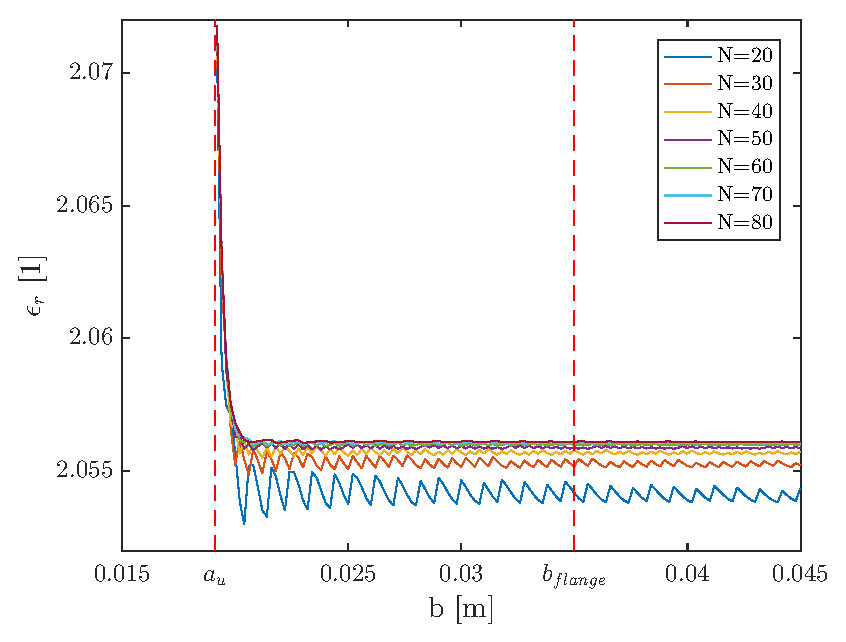
\includegraphics[scale=0.75]{b_conv_er.eps}
\caption{Convergence plot of the relative permittivity \er{} against the radius of the sample region $b$ (flange diameter). The convergence is plotted for different numbers of modes $N=20,30,40,50,60,70,80$, where $N$ refers to the number of modes in the upper cavity for optimum mode ratios (i.e. for optimum relative convergence). The resonant frequency used for the plot was \SI{9.6619}{\giga\hertz} and the thickness of the sample was \SI{1.509}{\milli\meter}. The upper cavity radius $a_u$ and the flange radius radius b\st{flange} are both marked with dashed vertical lines.}\label{fig:b_er}
\end{figure}

As shown above we can deal with the relative convergence phenomenon and ensure good convergence by choosing an optimum mode ratio for both models. But this on its own does not guarantee an accurate measurement, since the model must accurately model the field configuration in the split cylinder resonator. In Section \ref{sec:modelling} we have learnt that the split cylinder can be modelled as a closed cavity for certain modes like the TE\st{0np} modes, although it is in fact an open cavity. The region around the sample is a filled cylindrical cavity, which has a diameter of $2b$ and a length $d$. The fields in the gap of the open split-cylinder can be approximated with this filled cavity as long as we choose a diameter $2b$ that is large enough. For large diameters the electro-magnetic field in the sample region, measured at increasing distance from the origin, decays rapidly. So much, that for a certain diameter the conductive boundary at $\rho=b$ has no noticeable influence on the measurement any more. A plot of the dielectric constant (Fig. \ref{fig:b_er}) and the loss tangent (Fig. \ref{fig:b_tand}) against the radius of the sample region $b$ clearly shows that both converge rapidly if we increase the radius. If we vary the number of modes included in this computation, we can see that the convergence improves for increasing numbers of modes. Additionally, more modes also reduce the ripple of both the relative permittivity and the loss tangent. In this example, which is again our well-known PTFE sample, the relative permittivity and the loss tangent showed a ripple of around \num{2e-4} and \num{3.5e-7} for $N=30$ modes. For the number of modes that we used for most of our calculations $N=75$, the ripple became smaller than the uncertainties associated with the relative permittivity and the loss tangent. The ripple of the dielectric constant and loss tangent fell to \num{2.6e-5} and \num{1.2e-7}. These figures also show that the complex permittivity becomes stationary for $b>\SI{25}{\milli\meter}$, so we can choose any $b$ larger than \SI{25}{\milli\meter} without introducing any major error. Obviously, $b>\SI{25}{\milli\meter}$ yields a sufficiently accurate approximation of an open cavity for these two parameters. This does not necessarily mean that the field is approximated accurately, since the variational nature of the mode-matching method might suppress the influence of errors in the approximation. For our computations we decided to use the diameter of the flange of our prototype $2b_{flange}=\SI{70}{\milli\meter}$ as diameter of the sample region. 

\begin{figure}
\centering
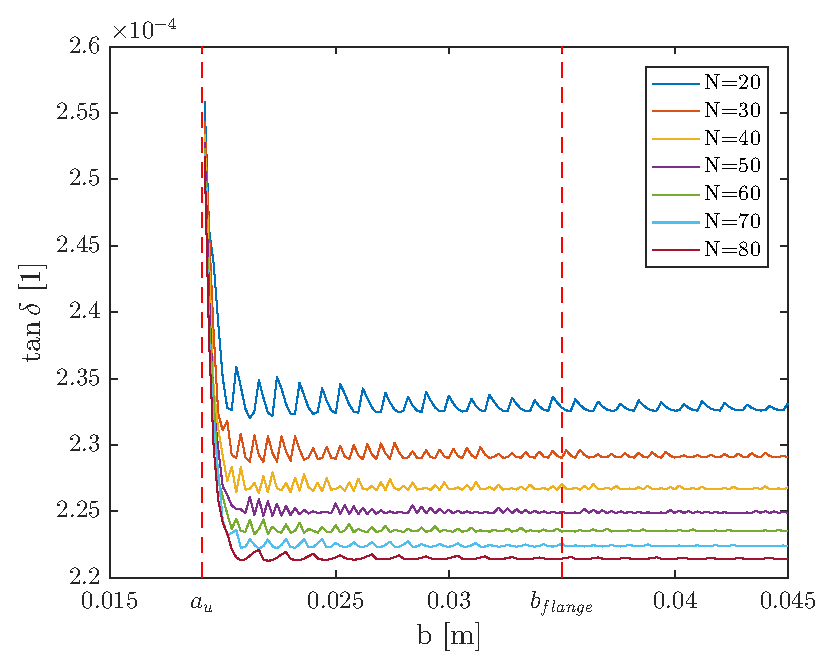
\includegraphics[scale=0.75]{b_conv_tand.eps}
\caption{Convergence plot of the loss tangent \tand{} against the radius of the sample region $b$ (flange diameter). The convergence is plotted for different numbers of modes $N=20,30,40,50,60,70,80$, where $N$ refers to the number of modes in the upper cavity for optimum mode ratios (i.e. for optimum relative convergence). The resonant frequency used for the plot was \SI{9.6619}{\giga\hertz}, the unloaded quality factor $Q_0$ of the resonance was \num{8754.3} and the thickness of the sample was \SI{1.509}{\milli\meter}. The upper cavity radius $a_u$ and the flange radius radius b\st{flange} are both marked with dashed vertical lines.}\label{fig:b_tand}
\end{figure}

\begin{figure}
\centering
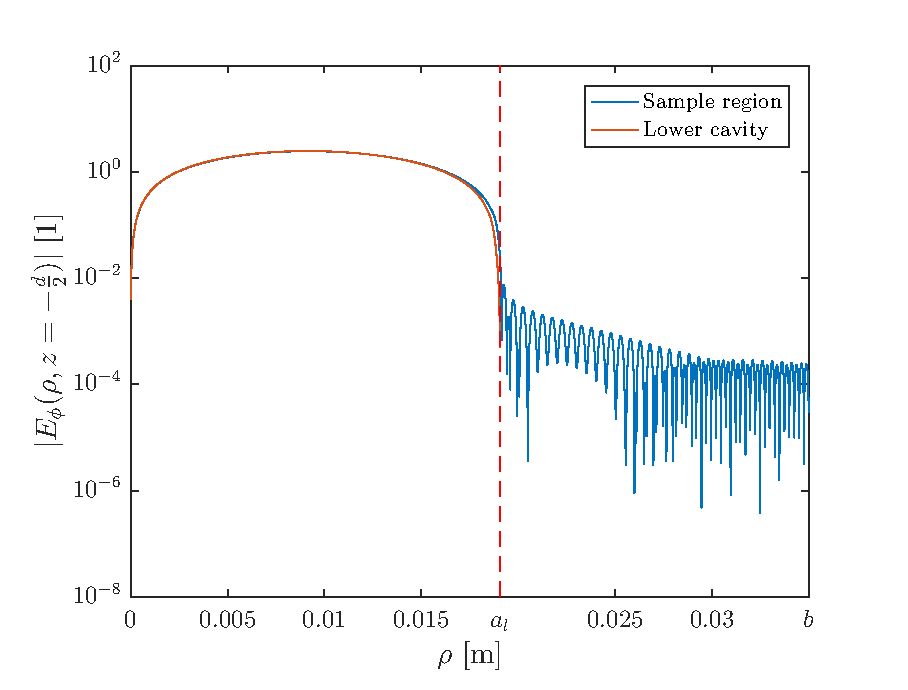
\includegraphics[scale=0.75]{E_phi_lower.eps}
\caption{M12 model - $\phi$ component of the normalised magnitude of the electric field for the sample region and for the lower cavity along their interface ($z=-\frac{d}{2}$). The radius of the lower cavity $a_l$ is marked with a dashed vertical line.}\label{fig:ephil}
\end{figure}
\begin{figure}
\centering
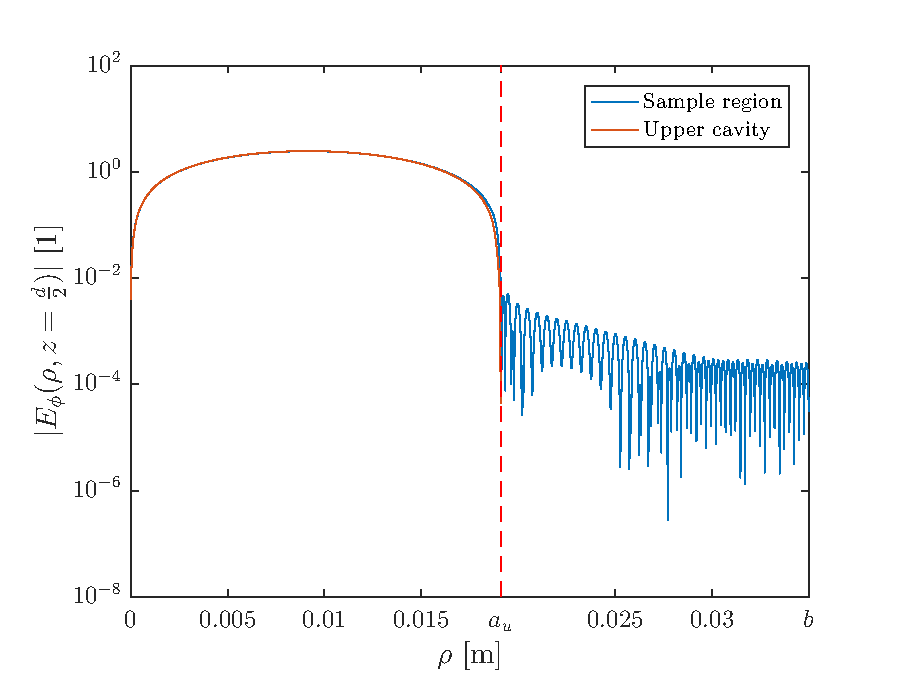
\includegraphics[scale=0.75]{E_phi_upper.eps}
\caption{M12 model - $\phi$ component of the normalised magnitude of the electric field for the sample region and for the upper cavity along their interface ($z=\frac{d}{2}$). The radius of the lower cavity $a_u$ is marked with a dashed vertical line.}\label{fig:ephiu}
\end{figure}

At the end of the last paragraph we mentioned that a sufficiently accurate approximation of the relative permittivity and the loss tangent of the resonator does not mean that the field in the resonator is approximated accurately. While our study of the relative convergence of the method clearly indicated that the functions of the relative permittivity and loss tangent are sufficiently smooth and converge to a true value with increasing numbers of modes, the underlying field configuration has not yet been examined. As the field in the resonator is a solution of the boundary-value problem of the split-cylinder resonator, we can check the field by looking at its boundary conditions. The boundary conditions that we need to check for this are not that of the perfectly conducting walls, which are naturally fulfilled by all modes in each region, but that of the interfaces. These are a figure of merit for how well the mode-matching method approximates the boundary value problem. As an example we examined the boundary conditions of a mode-matching calculation with $N=75$ modes that we made for the PTFE sample. Fig. \ref{fig:ephil} and \ref{fig:ephiu} illustrate that the tangential electric fields at both interfaces are very well matched. Over the entire aperture of each interface $0\leq\rho\leq a_{l,u}$ the electric fields on both sides are very similar and along the flange $a_{l,u}\leq \rho\leq b$ the electric field disappears as expected. As can be seen in Fig. \ref{fig:hrhol} and \ref{fig:hrhou} the magnetic field on the other hand is not very well matched at both interfaces. This is due to the conductor edges at $\rho=a_l$ and $\rho=a_u$ at the interface, which cause a singularity of the magnetic field (edge effect). A singularity causes a very rapid change in field strength, which cannot be approximated by the series expansions of the magnetic field. Similar to a Fourier series the spatial frequencies of the modes must be high enough to approximate a singularity. Another effect caused by the series expansion is the ripple of the approximations, which is also very similar to a Fourier series. Although the match of the magnetic field is relatively bad for this example, there is no need to worry. The magnetic field in this example is relatively weak at the boundary, so the singularity has a stronger influence on the field. Accordingly, the singularity also has less influence on the computed relative permittivity and loss tangent, as we have seen in the good convergence of the complex permittivity. The results for the calibration model were less suspicious: Fig. \ref{fig:ephical} and \ref{fig:hrhocal} show that both the tangential electric field $E_\phi$ and the tangential magnetic field $H_\rho$ were matched perfectly for the calbration, which was performed with a TE\st{011} mode at a resonant frequency of \SI{10.040}{\giga\hertz}.

\begin{figure}
\centering
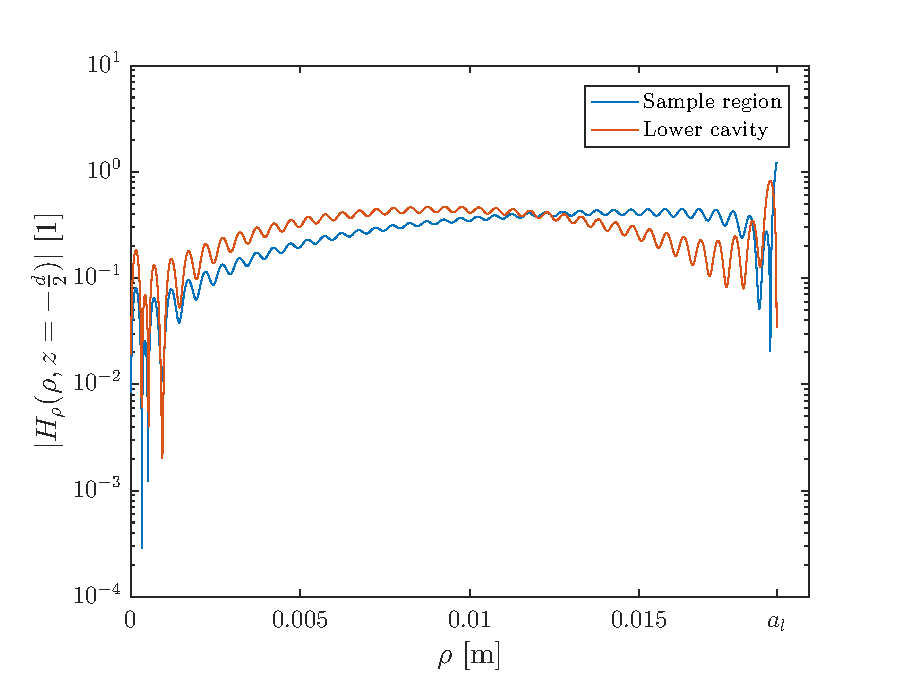
\includegraphics[scale=0.75]{H_rho_lower.eps}
\caption{M12 model - $\rho$ component of the normalised magnitude of the magnetic field for the sample region and for the lower cavity along their interface ($z=-\frac{d}{2}$).}\label{fig:hrhol}
\end{figure}
\begin{figure}
\centering
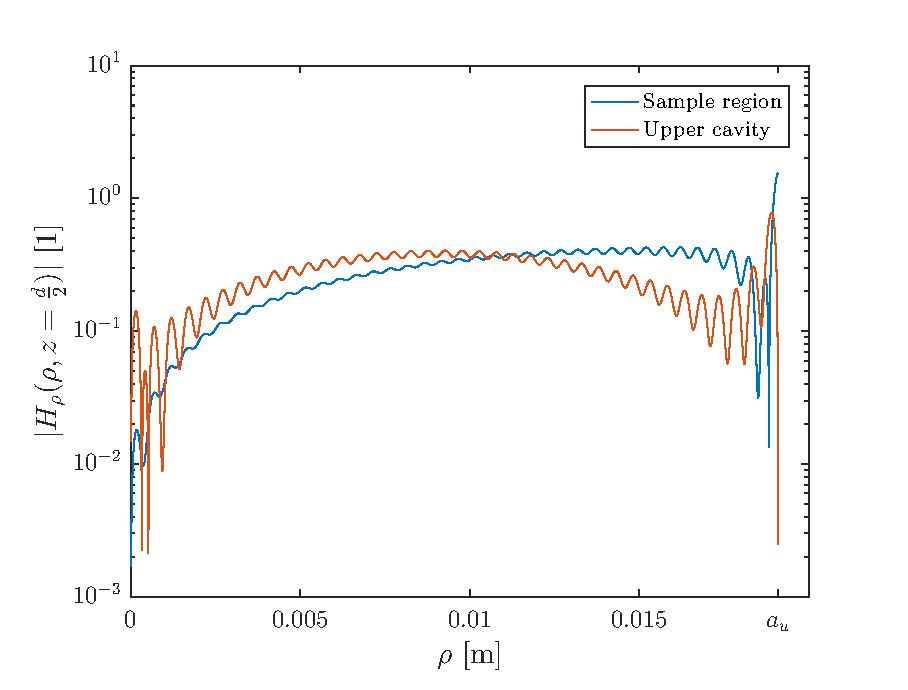
\includegraphics[scale=0.75]{H_rho_upper.eps}
\caption{M12 model - $\rho$ component of the normalised magnitude of the magnetic field for the sample region and for the upper cavity along their interface ($z=\frac{d}{2}$).}\label{fig:hrhou}
\end{figure}
\begin{figure}
\centering
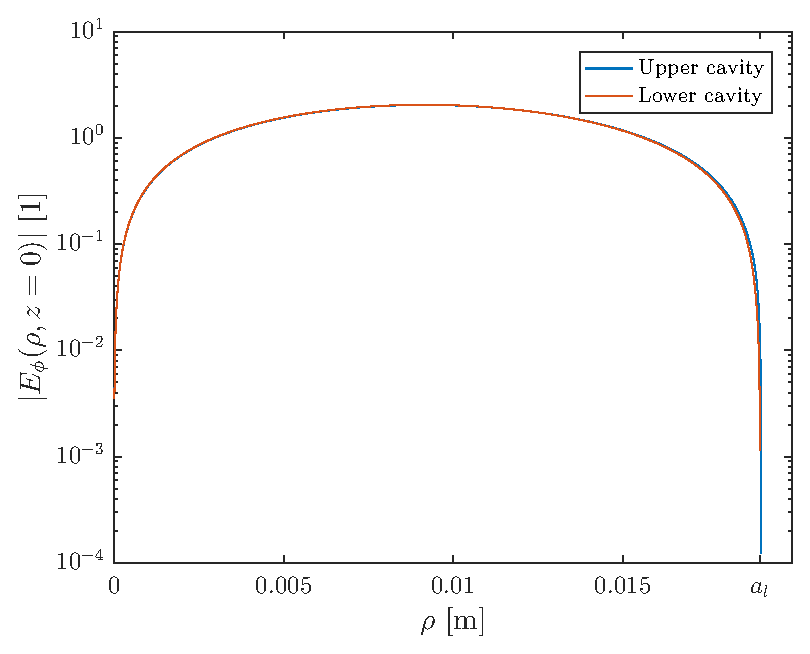
\includegraphics[scale=0.75]{E_phi_cal.eps}
\caption{Calibration model - $\phi$ component of the normalised magnitude of the electric field for the upper cavity and for the lower cavity along their interface ($z=0$).}\label{fig:ephical}
\end{figure}
\begin{figure}
\centering
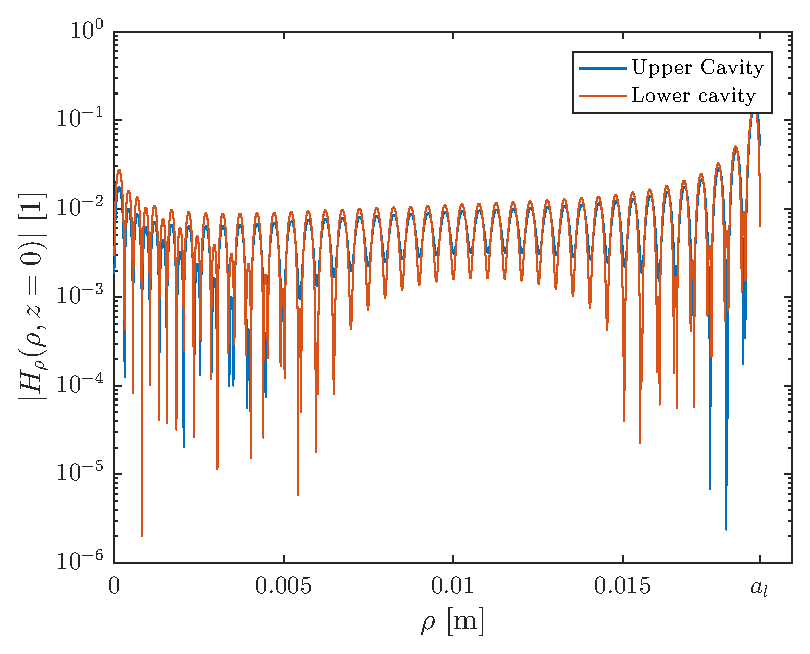
\includegraphics[scale=0.75]{H_rho_cal.eps}
\caption{Calibration model - $\rho$ component of the normalised magnitude of the magnetic field for the upper cavity and for the lower cavity along their interface ($z=0$).}\label{fig:hrhocal}
\end{figure}